\documentclass[class=book, crop=false, oneside, 12pt]{standalone}
\usepackage{standalone}
\usepackage{../../style}
\usepackage{csquotes}
\graphicspath{{./assets/images/}}

% arara: pdflatex: { synctex: yes, shell: yes }
% arara: latexmk: { clean: partial }
\begin{document}
\chapter{Analisi sintattica: top-down parsing}

\section{Il parsing}
Il parsing (o analisi sintattica) è quel processo in cui, data una grammatica \(\mathcal{G} = (V, T, S, \mathcal{P})\) e una parola \(w\), dobbiamo dire se \(w \in \mathcal{L(G)}\) e, se così fosse, fornire il suo albero di derivazione. Solitamente gli approcci al parsing che vengono presi in considerazione nell'ambito dei linguaggi di programmazione sono due: 
\begin{itemize}
    \item \textbf{Top-Down}: consiste nella costruzione di una derivazione leftmost da uno start symbol della grammatica e quindi procede dalla radice verso le foglie dell'albero di derivazione; a prima vista, si direbbe che sia l'approccio più intuitivo;
    \item \textbf{Bottom-Up}: consiste invece nella costruzione di una derivazione rightmost (in ordine inverso) della stringa dalle foglie alla radice.
\end{itemize}
A questo punto è necessario aggiungere che il parsing non si limita a questi due approcci, ma esiste anche in forma più generale utilizzando delle tattiche che vengono impiegate nel caso dei linguaggi naturali. Gli approcci descritti non permettono di considerare tutti i possibili linguaggi liberi, ma solamente delle sottoclassi: per questo si ha un'analisi sintattica estremamente efficiente dal punto di vista computazionale.

\subsection{Top-Down Parsing}
\subsubsection{Esempio 1}
Sia \(w\) = \(bd\) e sia \(\mathcal{G}\): 
\begin{align*}
    \mathcal{G}: S &\rightarrow Ad \mid Bd \\
    A &\rightarrow a \\
    B &\rightarrow b
\end{align*}

Per verificare se \(w \in \mathcal{L(G)}\) con un approccio top-down dobbiamo ottenere una derivazione leftmost a partire dallo start symbol. Ovviamente, si noterà subito che non è possibile scegliere \(Ad\) come derivazione iniziale dello start symbol, perché a quel punto l'unica parola ottenibile sarebbe parola \(ad\); dobbiamo invece optare per la seconda derivazione. La derivazione completa ci porta a
\begin{align*}
    S \Rightarrow Bd \Rightarrow bd
\end{align*}
Visto che abbiamo dimostrato che \(w \in \mathcal{L(G)}\) e che tale derivazione esiste, allora possiamo fornire il suo derivation tree che, per questo esempio, risulta davvero molto semplice.

\begin{figure}[H]
    \centering
    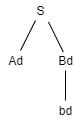
\includegraphics[width=.15\textwidth,keepaspectratio]{par-td-es1.png}
    \caption{Albero di derivazione per esercizio 1}
    \label{par-td-es1}
\end{figure}

\subsubsection{Esempio 2}
Sia \(w\) = \(id + id * id\) e sia \(\mathcal{G}\):
\begin{align*}
    \mathcal{G}: E &\rightarrow TE' \\
    E' &\rightarrow +TE' \mid \varepsilon \\
    T &\rightarrow FT' \\
    T' &\rightarrow *FT' \mid \varepsilon \\
    F &\rightarrow (E) \mid id
\end{align*}

Qui non è così intuitivo riuscire a dire se esiste una derivazione leftmost: che cosa mi conviene espandere? Avremo modo di parlare meglio di questo esempio non appena introdurremo il \textbf{Predictive top-down parsing}.

\subsubsection{Esempio 3}
Sia \(w\) = \(cad\) e sia \(\mathcal{G}\):
\begin{align*}
    S &\rightarrow cAd \\
    A &\rightarrow ab \mid a
\end{align*}

Nonostante questo esempio sia molto intuitivo, dobbiamo sforzarci di ragionare nei panni dell'algoritmo di parsing: dopo la prima derivazione, infatti, entrambe le opzioni che vengono proposte per poter derivare il non-terminale \(A\) sono apparentemente valide in quanto iniziano entrambe per \(a\). Quale delle due dovrei dunque scegliere? Quanto devo continuare l'esecuzione prima di accorgermi se ho fatto una scelta corretta oppure no? Il nostro algoritmo potrebbe anche trovarsi nel caso di dover fare \emph{backtrack}, perché semplicemente non c'era un modo semplice e generale per capire cosa dover scegliere: ovviamente questo tipo di tecnica funziona, ma vogliamo un approccio efficiente e il backtrack, come sappiamo, in questo non ci aiuta.

\subsection{Predictive Top-Down Parsing}
Nel caso del Predictive top-down parsing non è mai necessario applicare la tecnica del backtrack, poiché questo fa riferimento a una classe particolare di grammatiche, le quali vengono definite \textbf{LL(1) grammars}; vengono così chiamate per via della procedura impiegata per analizzarle, in cui:
\begin{itemize}
    \item guardiamo le parole da sinistra a destra;
    \item eseguiamo una produzione leftmost;
    \item guardiamo un solo simbolo (non-terminale).
\end{itemize}
Tali grammatiche prevedono una tipologia di parsing per cui non è necessario backtrack, e per di più è \textbf{completamente deterministica}.

Queste grammatiche vengono classificate a seconda del grado di determinismo che consentono; all'inizio del corso abbiamo visto la differenza tra le grammatiche senza contesto e contestuali, ma adesso le classi che incontreremo da oggi in poi si differenzieranno esclusivamente per il tipo di analizzatore con cui possiamo riconoscere le parole generate da queste grammatiche. 

In questo caso il parsing si basa sul fatto che possiamo costruire una tabella di parsing che ci guida nell'analisi della parola che ci viene data in input; quessta strategia ci permette molto efficacemente di dire se la parola appartenga oppure no al linguaggio e, in caso di esito positivo, di costruire la derivazione leftmost richiesta e il conseguente albero di derivazione.

Prendiamo come esempio il caso che abbiamo lasciato in sospeso precedentemente:
\begin{align*}
    \mathcal{G}: E &\rightarrow TE' \\
    E' &\rightarrow +TE' \mid \varepsilon \\
    T &\rightarrow FT' \\
    T' &\rightarrow *FT' \mid \varepsilon \\
    F &\rightarrow (E) \mid id
\end{align*}
\begin{table}[H]
	\centering
	\subimport{assets/tables/}{ptdp-example.tex}
    \caption{Tabella del parsing top-down}
    \label{ptdp-example}
\end{table} 
% \begin{figure}[H]
%     \centering
%     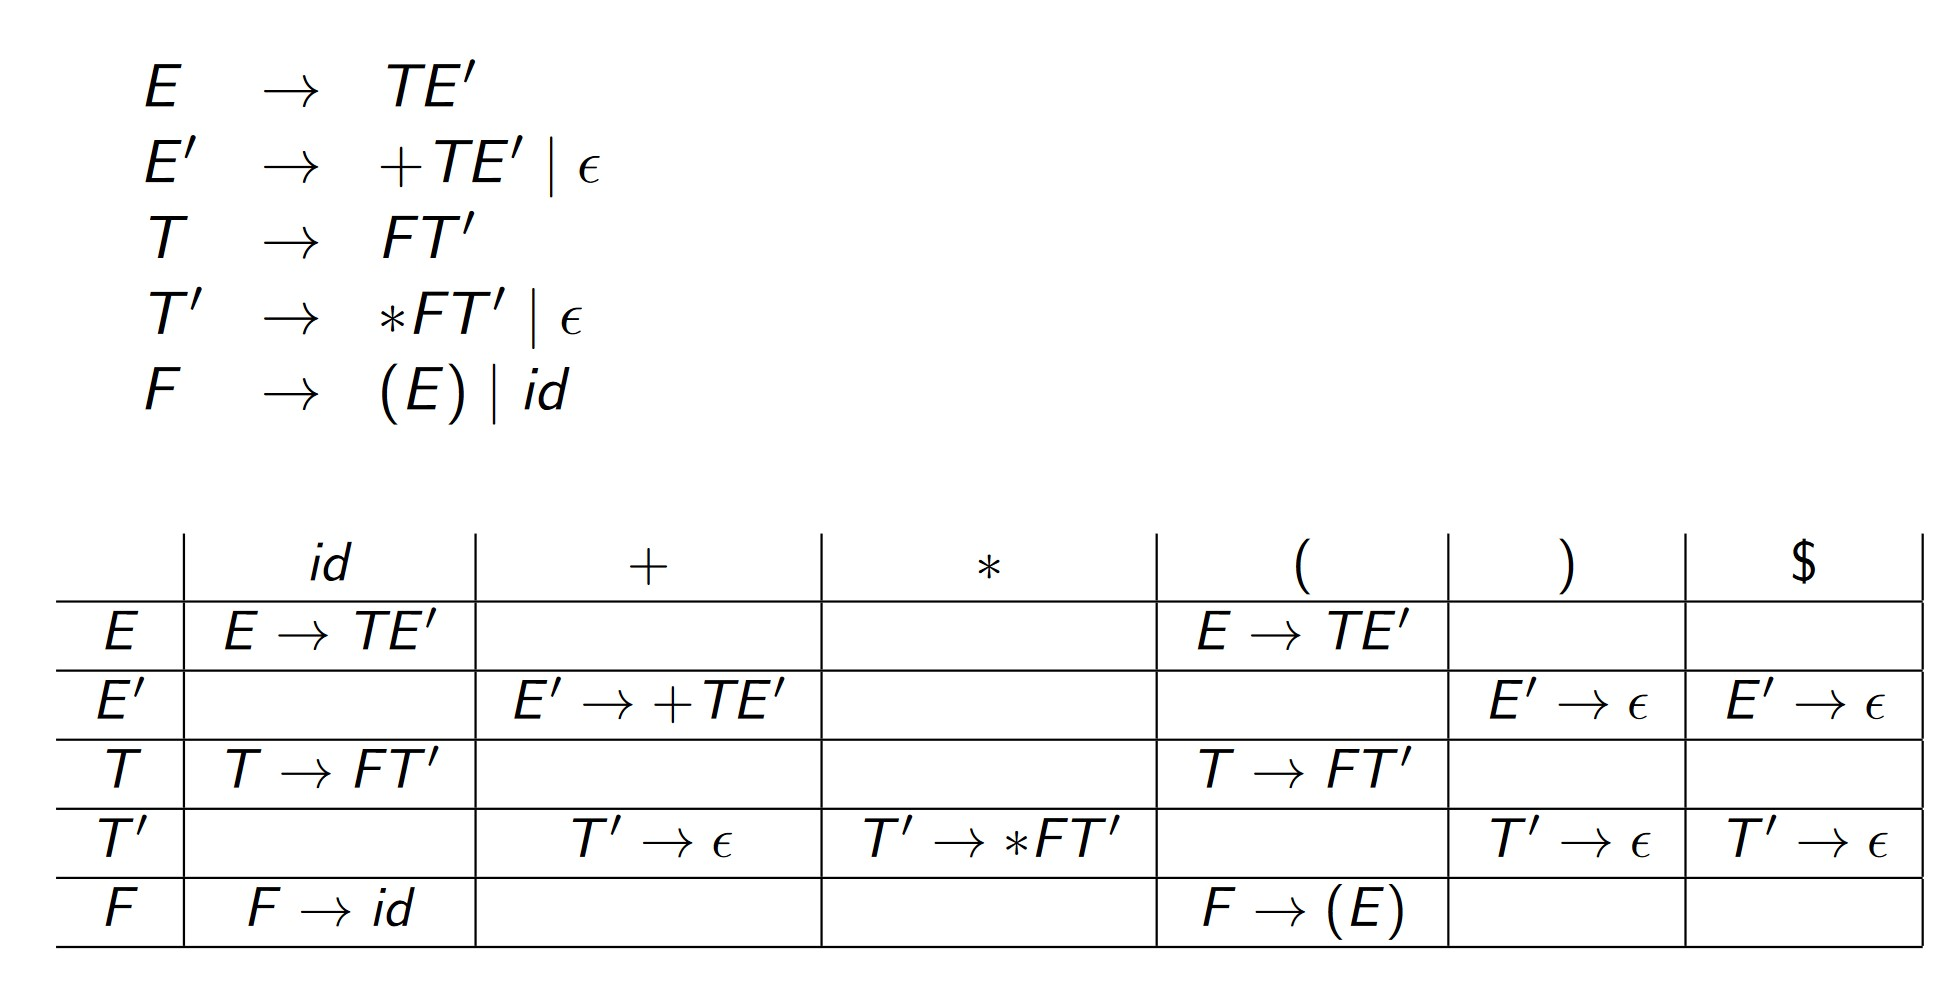
\includegraphics[width=.7\textwidth,keepaspectratio]{parsingTopDownTable.jpg}
%     \caption{parsingTopDownTable}
%     \label{parsingTopDownTable}
% \end{figure}

La tabella è così costruita:
\begin{itemize}
    \item si ha una \textbf{riga} per ogni non-terminale della grammatica;
    \item ed una \textbf{colonna} per ogni terminale della grammatica, a cui si aggiunge il simbolo \$ alla parola fornita in input e utilizzato come terminatore
    \item le entry vuote all'interno della tabella identificano i casi di errore.
\end{itemize}

Avendo a disposizione la tabella di parsing, la cui costruzione verrà trattata successivamente, è possibile utilizzarla per il parsing top-down predittivo.

\subsubsection{Algoritmo per il Predictive Top-Down Parsing}
\begin{itemize}
    \item Input: Una stringa \(w\), una tabella \(M\) di parsing top-down per la grammatica \(\mathcal{G} = (V, T, S, \mathcal{P})\);
    \item Output: La derivazione leftmost della stringa \(w \iff w \in \mathcal{L(G)}\), altrimenti \emph{error()}.
\end{itemize}
Inizializziamo la procedura posizionando \(w\$\) nell'input buffer e, nella pila che viene utilizzata per inserire e analizzare gli elementi parziali, inseriamo il simbolo \$ con lo start symbol \(S\) in cima.
\begin{figure}[H]
    \centering
    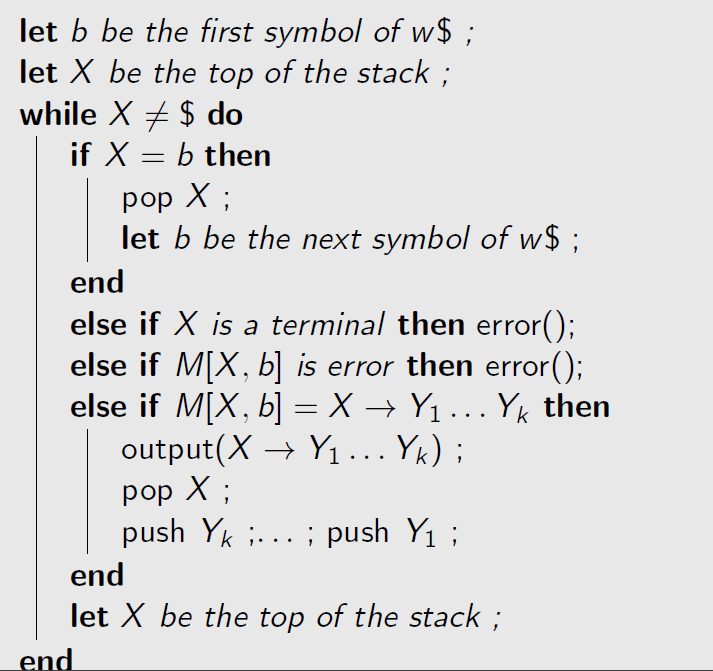
\includegraphics[width=.7\textwidth,keepaspectratio]{PredictiveTopDownAlgorithm.png}
    \caption{PredictiveTopDownAlgorithm}
    \label{PredictiveTopDownAlgorithm}
\end{figure}
\subimport{assets/pseudocode/}{pred-tdparsing.tex}

Nell'algoritmo di parsing si utilizza la variabile \(b\) come primo simbolo delle parola w\$ e si inizializza la variabile X con la cima dello stack (il caso base corrisponde ad avere \(X = S\)). Finché \(X \neq \$\) (sostanzialmente finché non ho svuotato completamente la pila), sono dati i seguenti casi:

\begin{enumerate}
    \item se \(X = b\), allora tolgo l'elemento dalla cima della pila e imposto \(b\) al simbolo successivo nell'input buffer. Questo corrisponde al caso in cui nella derivazione della costruzione parziale ho ottenuto un match con un terminale nella parola;
    \item se invece X è comunque un terminale, allora deve essere che \(X \neq b\), ma ciò produce un errore;
    \item se invece X è un non-terminale, allora è necessario verificare la tabella di top-down parsing in posizione \(M[X, b]\) e possono valere le seguenti:
    \begin{itemize}
        \item \(M[X, b]\) = \texttt{error} e allora viene restituito \texttt{error()};
        \item \(M[X, b] = X \rightarrow Y_1...Y_k\) e quindi è una produzione che verrà utilizzata per continuare la derivazione: questa viene stampata in output, viene rimosso l'elemento \(X\) dalla testa della pila e infine viene inserito il body della produzione in ordine inverso (cioè in modo che \(Y_1\) sia l'elemento in cima allo stack).
    \end{itemize}
\end{enumerate}

Infine, come ultima operazione \(X\) viene assegnato all'elemento in cima alla pila e si ripete. A seguire un esempio che fa uso dell'algoritmo appena descritto.
\begin{table}[htb]
	\centering
	\subimport{assets/tables/}{ptdp-ex1.tex}
    \caption{Tabella delle strutture a ogni passo}
    \label{ptdp-ex1}
\end{table} 
% \begin{figure}[H]
%     \centering
%     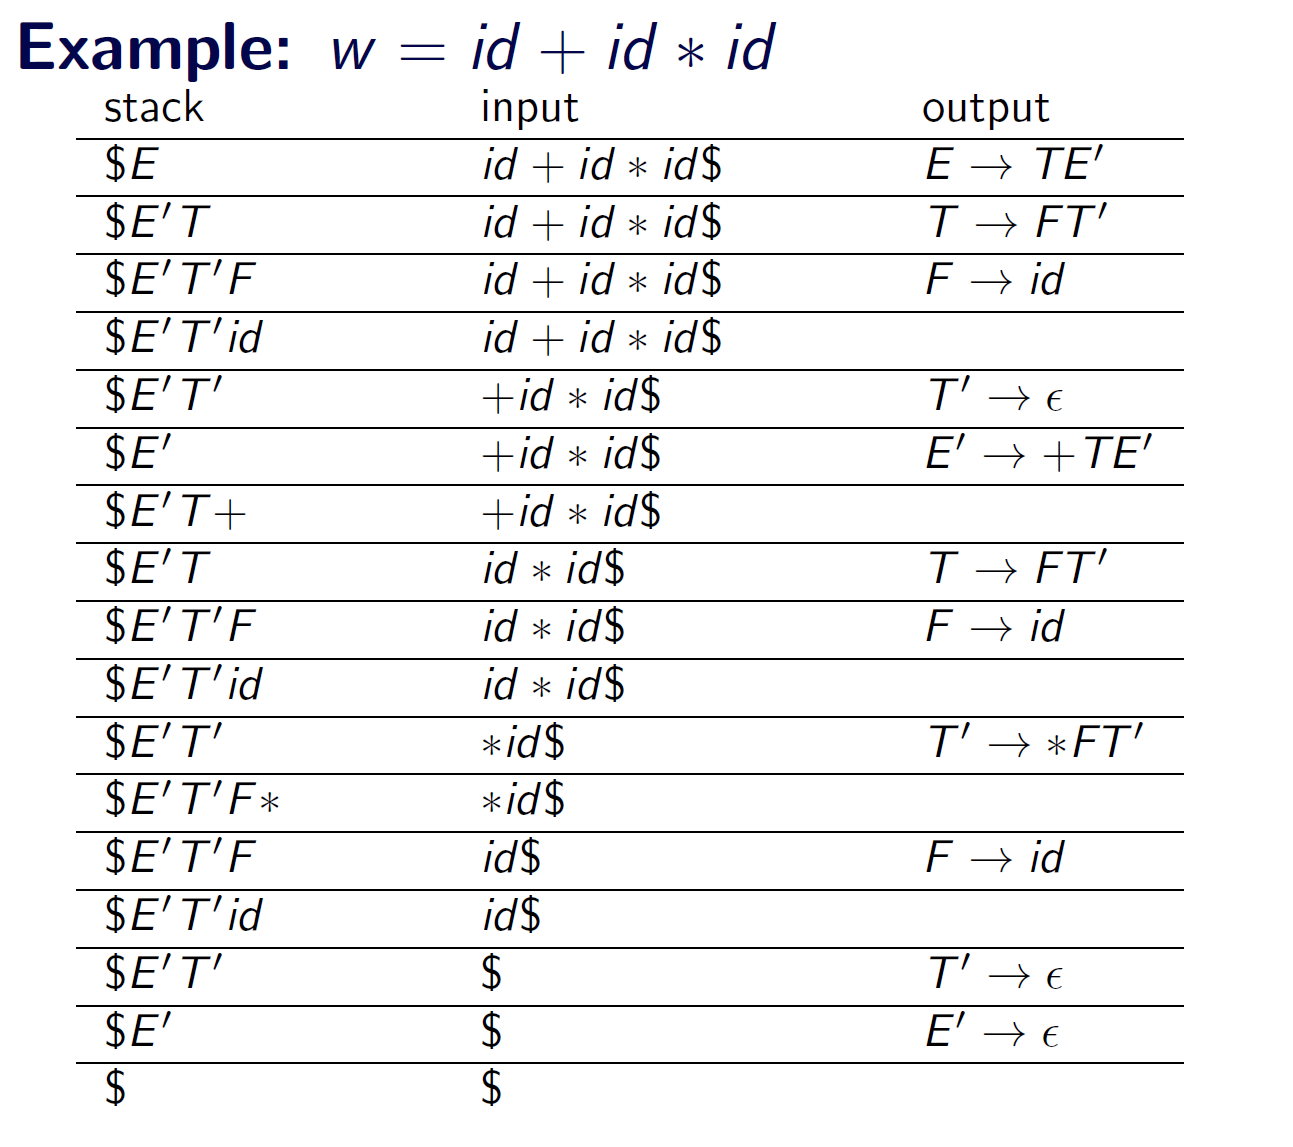
\includegraphics[width=.7\textwidth,keepaspectratio]{TopDownExercise.png}
%     \caption{TopDownExercise}
%     \label{TopDownExercise}
% \end{figure}

\subsection{Tabella di parsing}

L'algoritmo di Parsing predittivo ha una complessità lineare. Ci chiediamo quindi: come costruiamo le Parsing Table? In quale posizione dobbiamo mettere le produzioni della grammatica per fare sì che l'algoritmo funzioni?

Ricordiamo che la cella \(M[A, b]\) della parsing table viene consultata per espandere il non-terminale \(A\) sapendo che il prossimo terminale nell'input buffer è \(b\). Andiamo dunque a valorizzare la cella: \(M[A, b]\) = \(A \rightarrow \alpha\) se:

\begin{itemize}
    \item il body della nostra produzione di driver \(A\) è tale per cui esiste una derivazione del tipo \(\alpha \Rightarrow^* b \beta\), ossia partendo da \(\alpha\) si riesce, con zero o più passi, a ottenere una stringa che inizia per \(b\);
    \item oppure \(\alpha \Rightarrow^* \varepsilon\) ed è possibile avere \(S \Rightarrow^* w A \gamma\) (ottenuta da una derivazione di tipo leftmost) con \(\gamma \Rightarrow^* b \beta\)
\end{itemize}

Le celle per cui non è possibile inserire una produzione (cioè quelle vuote) verranno valorizzate a \texttt{error()}.

\subsubsection{Esercizio 1}

Sia data la seguente grammatica:
\begin{align*}
    \mathcal{G}: S &\rightarrow aA \mid bB \\
    A &\rightarrow c \\
    B &\rightarrow c
\end{align*}

Andiamo a vedere come costruire la tabella, aiutandoci dal fatto che è molto semplice ricavare a vista il linguaggio denotato dalla seguente grammatica, che include semplicemente le due parole \(ac\) oppure \(bc\). Partiamo dalle produzioni di \(S\):
\begin{itemize}
    \item se applichiamo la definizione precedente abbiamo che \(M[S, a] = S \rightarrow aA\), in quanto solamente utilizzando quella produzione riusciremmo ad avere una stringa che comincia per \(a\) (\(aA \Rightarrow ac\));
    \item lo stesso ragionamento può essere applicato per \(M[S, b] = S \rightarrow bB\);
    \item dal momento che non è possibile creare delle stringhe che cominciano per il terminale \(c\), allora avremo che \(M[S, c] = error()\);
\end{itemize}
A questo punto è possibile passare agli altri due non-terminali della grammatica: 
\begin{itemize}
    \item nel caso di \(A\) è possibile notare che esiste una sola produzione che permette di ottenere soltanto \(c\), quindi avremo che \(M[A, c] = A \rightarrow c\);
    \item nel secondo caso è possibile applicare la stessa logica, per cui avremo che \(M[B, c] = B \to c\).
\end{itemize} 
La tabella finale sarà quindi costruita in questo modo:

\begin{table}[H]
	\centering
	\subimport{assets/tables/}{filling-parsing-table1.tex}
    \caption{Parsing table per esercizio 1}
    \label{filling-parsing-table1}
\end{table} 

Ricordiamoci che non è possibile che più produzioni possano essere inserite all'interno della stessa cella, in quanto ci stiamo occupando delle grammatiche LL1, nelle quali è possibile applicare un parsing di tipo deterministico. 

Quando si arriva ad una error entry vuol dire che sulla testa della pila c'è un non-terminale che, indipendentemente da come decida di espanderlo, non mi porterà mai alla stringa che sto cercando di ottenere. 

\subsubsection{Esercizio 2}
Sia data la seguente grammatica:
\begin{align*}
    \mathcal{G}: S &\rightarrow aAb \\
    A &\rightarrow \varepsilon
\end{align*}

In questo esempio, invece, il linguaggio denotato dalla nostra grammatica è composto solamente dalla parola \(ab\). Per la definizione di \(\alpha\), l'unica cella che ha come non-terminale (nonché start symbol) \(S\) è la cella \(M[S, a] = S \rightarrow aAb\), perché l'unica stringa che è possibile ottenere inizia per \(a\). Da qui è possibile intuire anche che, per ottenere la parola \(ab\), è necessario che \(M[A, b] = S \rightarrow \varepsilon\); in tutti gli altri casi verrà ritornato un errore, in quanto tale parola non apparterrebbe al linguaggio denotato dalla grammatica. 

\begin{table}[H]
	\centering
	\subimport{assets/tables/}{filling-parsing-table2.tex}
    \caption{Parsing table per esercizio 2}
    \label{filling-parsing-table2}
\end{table}

\section{First(\(\alpha\))}
\subsection{Definizione}
\begin{definition}
    Chiamiamo \(first(\alpha)\) quell'insieme di terminali che sono posti all'inizio delle stringhe derivate da \(\alpha\).
    
    Inoltre, se \(\alpha \Rightarrow^* \varepsilon\), allora \(\varepsilon \in \textrm{first}(\alpha)\): ciò vuol dire che \(\alpha\) è un non-terminale annullabile (nullable) e quindi, dopo una serie di passi, sarà pari a \(\varepsilon\).
\end{definition}

Il concetto di first può essere definito ricorsivamente come segue:

\begin{labeling}{step}
    \item[base] casi base:
    \begin{itemize}
        \item first(\(\varepsilon\)) = \{\(\varepsilon\)\}
        \item first(\(a\)) = \{\(a\)\}
    \end{itemize}
    \item[step] first(\(A\)) = \(\cup_{A \rightarrow \alpha}\) first(\(\alpha\))
\end{labeling}

    Nell'ultimo caso, quello ricorsivo, si ha che first(\(A\)) è dato dall'unione di tutti i first(\(\alpha\)), dove \(\alpha\) è il body delle produzioni della grammatica che hanno \(A\) come driver.

\subsection{Algoritmo di calcolo di first(\(\alpha\))}

Mostriamo ora un algoritmo che ci permette di calcolare first(\(Y_1 \ldots Y_n\)) (con \(Y_i \in V\)), cioè l'insieme dei first per una certa parola considerata.

\begin{figure}[H]
    \centering
    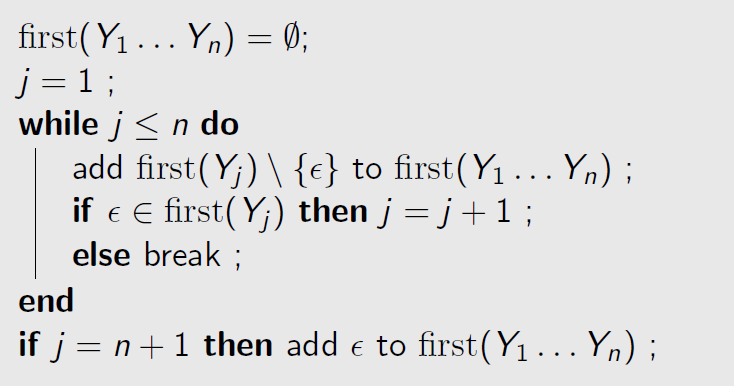
\includegraphics[width=.7\textwidth,keepaspectratio]{first-algorithm.png}
    \caption{Algoritmo per calcolare first(\(\alpha\))}
    \label{first-algorithm}
\end{figure}
\subimport{assets/pseudocode/}{first.tex}

Andiamo a vedere più da vicino quale idea stiamo seguendo in questo algoritmo. Dopo aver inizializzato l'insieme dei first(\(Y_1 \ldots Y_n\)), vado a iterare su tutti gli elementi \(Y_j \in V\) della parola: 
\begin{itemize}
    \item finché non abbiamo esaminato tutti gli \(Y_j : 1 \leq j \leq n\), si aggiunge first(\(Y_j\)) \(\setminus\{\varepsilon\}\) ai first(\(Y_1 \ldots Y_n\)) e poi si controlla se \(\varepsilon \in\) first(\(Y_j\));
    \item se il controllo restituisce \texttt{true}, allora vuol dire che è necessario continuare la ricerca dei first, perché è possibile che in almeno un caso \(Y_j = \varepsilon\) e quindi è possibile che nessuno dei first(\(Y_j\)) \(\in\) first(\(Y_, \ldots Y_n\));
    \item se il controllo restituisce invece \texttt{false}, allora possiamo fermarci, in quanto abbiamo trovato tutti i first(\(Y_1, \ldots, Y_n\)).
\end{itemize} 
L'ultimo controllo serve per verificare se, \(\forall\) \( Y_j \in (Y_1 \ldots Y_n)\), non sono in realtà tutti annullabili; in tal caso, sarebbe necessario aggiungere anche \(\varepsilon\) ai first(\(Y_1 \ldots Y_n\)), in quanto \((Y_1 \ldots Y_n)\) sarebbe annullabile.

\subsection{Training}
Sia data la seguente grammatica:
\begin{align*}
    \mathcal{G}: E &\rightarrow TE' \\
    E' &\rightarrow +TE' \mid \varepsilon \\
    T &\rightarrow FT' \\
    T' &\rightarrow *FT' \mid \varepsilon\\
    F &\rightarrow (E) \mid id
\end{align*}

L'idea generale è quella dunque di partire dai casi base, vale a dire da quelle produzioni che hanno come body o un terminale oppure \(\varepsilon\). Nel nostro caso dunque, secondo la definizione espressa precedentemente, possiamo risolvere immediatamente la procedura per i seguenti casi: 
\begin{align*}
    \{\varepsilon\} &\in first(E')\textrm{,} &\textrm{da}\; E' &\to \varepsilon \\
    \{\varepsilon\} &\in first(T')\textrm{,} &\textrm{da}\; T' &\to \varepsilon \\
    \{id\} &\in first(F)\textrm{,} &\textrm{da } F\; &\to id
\end{align*}

A questo punto dobbiamo applicare l'algoritmo per ogni produzione: ad esempio, per calcolare first(\(F\)) dobbiamo fare l'unione di tutte le produzioni di \(F\); nel nostro caso saranno quindi \(F \rightarrow (E) \cup F \rightarrow id\):
\begin{itemize}
    \item nel primo caso abbiamo \((E)\), che è una parola composta di tre elementi (\(Y_1 = '(', Y_2 = E, Y_3 = ')'\), il lettore perdoni l'abuso di notazione nell'utilizzo degli apici) e dunque per prima cosa dobbiamo analizzare first(\(Y_1\)); tuttavia, \(Y_1 = '('\) è un terminale, da cui avremo che il suo first sarà first(\(Y_1\)) = \{\(Y_1\)\}, il che significa che \(\{Y_1\} \neq \varepsilon\), per cui possiamo aggiungerlo a first(\(F\)) e fermiamo subito l'algoritmo;
    \item nel secondo caso, invece, ci troviamo di fronte al caso base first(\(id\)) = \(\{id\}\) e dunque possiamo subito aggiungerlo a first(\(F\)).
\end{itemize}
In questo caso il risultato finale è dunque first(\(F\)) = \(\{(\} \cup \{id\} = \{(, id\}\).

A questo punto, il miglior modo per procedere nell'algoritmo è, in mancanza di casi base, trovare una produzione del tipo \(A \rightarrow F\alpha\); in questo modo possiamo sfruttare la conoscenza appena ottenuta relativamente a first(\(F\)). Applicando dunque l'algoritmo per first(\(T\)) è necessario analizzare \(T \rightarrow FT' = Y_1Y_2\), quindi andiamo a controllare per primo first(\(Y_1\)). Dal momento che che abbiamo già calcolato first(\(F\)) e poiché \(\varepsilon \notin\) first(\(F\)), possiamo direttamente arrestare l'algoritmo e affermare che first(\(T\)) = first(\(T\)) = \(\{(, id\}\).

Svolgendo dunque l'esercizio nella sua interezza è possibile ottenere il seguente risultato:

\begin{table}[H]
	\centering
	\subimport{assets/tables/}{computing-first.tex}
    \caption{Esercizio sui first}
    \label{computing-first}
\end{table}

Cosa sarebbe successo se invece la produzione di \(T\) fosse stata \(T \to T’F\)? Se tutto ill resto rimane invariato, dobbiamo andare a rivedere l'insieme first(\(T\)). Al posto dei first(\(F\)), in questo caso avremo i first(\(T’\)), per cui otterremo \(\{\varepsilon, \ast\}\); dal momento che \(\varepsilon\) è contenuto nell'insieme, l’algoritmo non si ferma (e non aggiunge ancora \(\varepsilon\) ai first(\(T\)) e procediamo quindi ad aggiungere ai first(\(T\)) anche i first(\(F\)), che sono \(\{id, )\}\); a questo punto i first non contengono \(\varepsilon\) e quindi termino riportando come first(\(T\)) \(\{\ast, id, )\}\)

\section{Follow(\(A\))}
\subsection{Definizione}
A differenza dei first, che sono definiti per stringhe generiche di terminali e non-terminali, i \emph{follow} sono computati solamente per i non-terminali infatti scriveremo follow(\(A\)).
\begin{definition}
    Con follow(\(A\)) indichiamo l'insieme dei terminali che possono seguire A in qualche derivazione.    
\end{definition}
I first evidenziano quali sono i terminali per cui iniziano le stringhe derivabili da certi elementi (stringhe o non-terminali), i follow invece indicano quali sono i terminali che possono seguire.

\subsection{Algoritmo per il calcolo dei follow(\(A\))}

\begin{figure}[H]
    \centering
    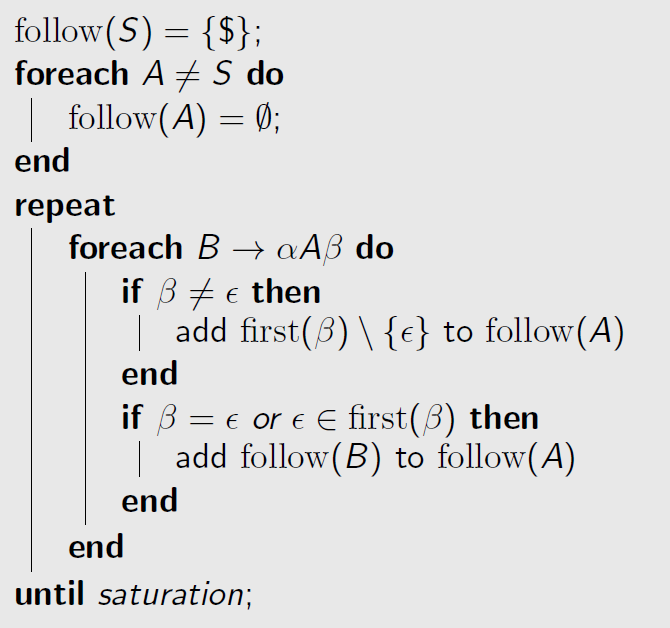
\includegraphics[width=.7\textwidth,keepaspectratio]{follow-algorithm.png}
    \caption{Algoritmo per calcolare follow(\(A\))}
    \label{follow-algorithm}
    % PER CHI RISCRIVERà L'ALGORITMO: lasciate la label invariata o fate un refactoring perché viene referenziata giù dabbasso <3
    % np l'ho cambiata anche dabbasso <3
\end{figure}
\subimport{assets/pseudocode/}{follow.tex}

L'algoritmo comincia impostando follow(\(S\)) = \$, dal momento che lo start symbol genera tutte le possibili parole, e per qualsiasi parola possiamo aspettarci di trovare il terminatore di stringa \$. Negli altri casi, invece, \(\forall A\) tale che \(A\) è un non-terminale, inizializziamo in questo modo: follow(\(A\)) = \(\emptyset\).

A questo punto è necessario sottoloneare che ci interessano solamente le produzioni della grammatica per cui il simbolo \(A\) non compare come driver della grammatica, ma come body; dunque, per ogni \(B \rightarrow \alpha A \beta\), si eseguono le sequenti operazioni: 

\begin{itemize}
    \item se \(\beta \neq \varepsilon\), allora aggiungiamo first(\(\beta\)) \(\setminus \varepsilon\) a follow(\(A\));
    \item se \(\beta = \varepsilon\) or \(\varepsilon \in\) first(\(\beta\)), allora aggiungiamo follow(\(B\)) a follow(\(A\)), perché quello che segue \(B\) potrà seguire anche \(A\) (si tenga presente che se \(\beta = \varepsilon\), allora \(A\) è la radice dell'ultimo sottoalbero generato da \(B\).
\end{itemize}   
% se si immagina un albero di derivazione qusto è formato da un sottoalbero per alpha, poi abbiamo un sottoalbero di A e poi quello di beta che contiene tutto quello che derivad a beta: tutti i terminali che sono diversi da epsilon e derivano da beta allora li mettiamo in A. Se invece beta è uguale a epsilon oppure epsilon appartiene ai first di beta allora dobbiamo aggiungere i follow di B ai follow di A perchè ciò che segue B potrà anche seguire A perchè se noi andiamo a considerare i sottoalberi che vengono generati andiamo a scoprire che A è la radice dell'utlimo sottoalbero della B e quindi quello che può seguire questa particolare occorrenza di B ... Si procede aggiungendo degli elementi ogni volta che andiamo a considerare delle partciolari istanze nella nostra grammatica e ci fermiamo fino a quando non possiamo inserire altro. 
\subsection{Training: esercizi su first/follow}
\subsubsection{Esercizio first/follow 1}
Utilizziamo sempre la grammatica dell'esempio precedente, che qui riportiamo per comodità del lettore, e andiamone a definire i follow.
\begin{align*}
    \mathcal{G}: E &\rightarrow TE' \\
    E' &\rightarrow +TE' \mid \varepsilon \\
    T &\rightarrow FT' \\
    T' &\rightarrow *FT' \mid \varepsilon\\
    F &\rightarrow (E) \mid id
\end{align*}
\begin{enumerate}
    \item Dall'algoritmo sappiamo follow(\(E\)) = \$;
    \item iniziamo guardando la prima produzione, cioè \(E \rightarrow TE'\): se poniamo \(A = E'\), allora \(\beta = \varepsilon\) dunque devo aggiungere i follow(\(E\)) (quelli del driver) a follow(\(E'\)) (quelli del body);
    \item Sempre soffermandoci sulla stessa produzione poniamo \(A = T\), questo vuol dire che \(\beta = E' \neq \varepsilon\) e quindi, ricadendo nel primo caso, aggiungo first(\(E'\)) \(\setminus \{\varepsilon\} = \{+\}\) a follow(\(T\)), tuttavia, essendo che \(\varepsilon \in\) first(\(E'\)) allora ricadiamo anche nel secondo caso per cui aggiungiamo follow(\(E\)) a follow(\(T\));
    \item Passiamo ora alla produzione \(E' \rightarrow +TE' \mid \varepsilon\): poniamo quindi \(A = E'\) e, essendo che \(\beta = \varepsilon\) ricadiamo nel secondo caso dunque dobbiamo aggiungere follow(\(E'\)) a follow(\(E'\)): dato che questo non fornisce informazioni aggiuntive scartiamo questa informazione;
    \item Possiamo ora esaminare il caso per la produzione precedente, in cui \(A = T\) e quindi \(\beta = E'\), ma tale caso è già stato esaminato al punto 3;
    \item L'ultimo elemento che non abbiamo esaminato nella produzione è terminale \(+\) ma, in quanto terminale, non possiamo calcolarne i follow(\(+\));
    \item Continuiamo ad applicare l'algoritmo come visto nei punti precedenti per computare i follow delle produzioni rimanenti;
    \item Un caso che potrebbe risultare interessante riguarda la produzione \(F \rightarrow (E)\). Poniamo come fatto precedentemente \(A = E\) e, essendo che \(\beta = (\) \(\neq \varepsilon\), è necessario aggiungere first(\(\beta\)) \(\setminus \{\varepsilon\} = \{)\}\) a follow(\(E\)) e, visto che la seconda condizione non è vera, possiamo fermarci ed affermare che follow(\(E\)) = \{\$, )\}.
\end{enumerate}
Il risultato finale verrà rappresentato come segue:
\begin{table}[H]
	\centering
	\subimport{assets/tables/}{computing-follow.tex}
    \caption{Esercizio sui follow, step intermedio}
    \label{computing-follow}
\end{table}

A questo punto è possibile eliminare mano a mano le dipendenze e le varie ripetizioni presenti all'interno delle computazioni dei follow, in modo da ottenere quanto segue: 

\begin{table}[H]
	\centering
	\subimport{assets/tables/}{follow.tex}
    \caption{Esercizio sui follow, risultato finale}
    \label{follow}
\end{table}

\subsubsection{Esercizio first/follow 2}
\label{first-folllow-ex-2}
Prendiamo ora in analisi la seguente grammatica:
\begin{align*}
       \mathcal{G}: S &\to aABb \\
       A &\to Ac \mid d \\
       B &\to CD \\
       C &\to e \mid \varepsilon \\
       D &\to f \mid \varepsilon
\end{align*}
Questa volta ripassiamo anche il calcolo dei first.
\begin{enumerate}
    \item Partiamo da \(S\): per calcolare i first di un non-terminale andiamo a vedere i first di tutte le sue produzioni; in particolare, so che qualunque stringa derivata da \(S\) inizierà con \(a\), e siccome \(a\) è un terminale ed è diverso da \(\varepsilon\), non proseguo oltre nella ricerca di first per \(S\);
    \item per calcolare i first di \(A\), invece, ho due produzioni da vagliare: la prima (che derivo da \(A \to Ac\)) mi dice che i first di \(A\) contengono anche i first dello stesso \(A\) (non aggiunge informazioni), la seconda mi dice che \(d\) può essere un first di \(A\), quindi scrivo \(\{d\}\);
    \item per calcolare i first di \(B\) devo conoscere quelli di \(C\) e \(D\), e dunque parto da \(C\): ottengo semplicemente che i first sono \(\{e\}\) e possibilmente \(\{\varepsilon\}\), quindi per \(C\) scrivo \(\{e, \varepsilon\}\);
    \item in modo simile a \(C\) posso facilmente ricavare che i first di \(D\) sono \(\{f, \varepsilon\}\);
    \item tornando ora ad analizzare \(B\) posso dire che i suoi first sono first(\(C\)) \( \setminus \{\varepsilon\}\), ma siccome \(C\) contiene \(\varepsilon\) tra i suoi first, allora devo aggiungere first(\(D\)) a first(\(B\));
    \item infine, notando che anche first(\(D\)) contiene \(\varepsilon\), posso annoverare in first(\(B\)) anche \(\varepsilon\) stesso.    
\end{enumerate}
Ora che abbiamo terminato la nostra ricerca dei first possiamo ricavare la tabella risolutiva dell'esercizio, che si presenta come in Tab. \ref{first-follow-ex-2_step-1}.
\begin{table}[H]
	\centering
	\subimport{assets/tables/}{first-follow-ex-2_step-1.tex}
    \caption{Esercizio \ref{first-folllow-ex-2} su first/follow, step 1}
    \label{first-follow-ex-2_step-1}
\end{table}
Passiamo ora gaiamente al prossimo step, ovvero il calcolo dei vari follow seguendo l'algoritmo indicato in Alg. \ref{alg:follow}.

Per comodità notazionale, dato che nelle produzioni dell'esercizio compare il non-terminale \(A\), scriveremo \(X\) per indicare la \(A\) dell'algoritmo per il calcolo del follow (assumiamo quindi che ogni \(A\) nell'algoritmo venga sostituita da \(X\); quindi, ad esempio, \(\alpha A \beta\) diventa \(\alpha X \beta\)).
\begin{enumerate}
    \item la fase di inizializzazione del calcolo dei follow vuole che lo start symbol abbia come follow il terminatore di stringa, per le ragioni che abbiamo già visto, quindi inseriamo subito \(\$\) per \(S\);
    \item cominciamo poi l'analisi dalle produzioni di \(S\):
    \begin{enumerate}
        \item osservando l'algoritmo, cerchiamo un match possibile per \(\alpha X \beta\); partiamo con il considerare \(X\) = \(A\) e quindi consideriamo \(\beta\) = \(Bb\);
        \item in questo caso abbiamo che \(\beta \neq \varepsilon\), quindi dobbiamo aggiungere i first(\(\beta\)) ai follow(\(A\));
        \item i first di \(\beta\) in questo caso sono i first di \(Bb\), quindi \(\{e, f, b\}\) (nota bene che non sono first(\(B\)) ma first(\(Bb\))); come indicato nella procedura, li aggiungo a follow(\(A\));
        \item \(\beta\) è diverso da \(\varepsilon\) ed il suo first non contiene \(\varepsilon\), quindi il secondo \texttt{if} non si applica e terminiamo questo branch;
        \item ora dobbiamo analizzare il caso in cui, studiando la produzione di \(S\), assumiamo \(X = B\) e quindi \(\beta = b\);
        \item in questo caso ho che devo aggiungere ai follow di \(B\) i first(\(b\)), ovvero \(\{b\}\);
        \item \(\beta\) è diverso da \(\varepsilon\) ed inoltre \(\varepsilon\) non appartiene ai first di \(\beta\), quindi termino anche questo branch.
    \end{enumerate}
    \item Ho concluso quindi l’analisi delle produzioni di \(S\) e passo quindi ad analizzare la produzione di \(A\):
    \begin{enumerate}
        \item parto da \(A \to Ac\): in questo caso non ho altra scelta che considerare \(X = A\), quindi \(\beta = c\) e cado quindi nel primo \texttt{if} dell'algoritmo, il quale mi dice di aggiungere first(\(c\)) \(\setminus \{\varepsilon\}\) (ovvero \(\{c\}\)) ai follow(\(A\));
        \item chiudo quindi il branch dato che il secondo \texttt{if} non si applica;
        \item considero ora la seconda produzione di \(A\), ovvero \(A \to d\); tuttavia, questa non è nella forma \(\alpha X \beta\) e quindi non ci dà informazioni, per cui l'algoritmo mi dice che posso passare oltre; ho terminato le produzioni di \(A\).
    \end{enumerate}
    \item Passiamo all'analisi della produzione \(B \to CD\):
    \begin{enumerate}
        \item considero \(X = C\) e ottengo quindi \(\beta = D\), e dato che \(\beta \neq \varepsilon\) aggiungo ai follow(\(C\)) i first(\(D\))\( \setminus \{\varepsilon\} = \{f\}\);
        \item però, dal momento che \(\varepsilon \in \) first(\(\beta\)), cado nel secondo \texttt{if} e devo quindi aggiungere i follow(\(B\)) (inteso come \(B\) dell'algoritmo) ai follow(\(X\)), il che significa aggiungere i follow(\(B\)) ai follow(\(C\)) nel nostro esercizio; lascio quindi un placeholder nella tabella da riscrivere quando avrò finito di calcolare follow(\(B\)), avendo raggiunto la fine del ciclo \texttt{while} chiudo qui il branch;
        \item ora considero la seconda opzione, ovvero \(X = D\), quindi \(\beta = \varepsilon\);
        \item in questo caso andiamo direttamente nel secondo \texttt{if} che ci dice di aggiungere i follow(\(B\)) ai follow(\(D\)); nella tabella, quindi, indico un altro placeholder;
        \item abbiamo terminato le possibili interpretazioni delle produzioni per la derivazione \(B \to CD\).
    \end{enumerate}
    \item Le produzioni di \(C\), come quelle di \(D\), non sono del tipo \(\alpha X \beta\), dato che non contengono caratteri non-terminali; queste produzioni non ci danno informazioni sui follow e l’algoritmo ci dice pertanto di ignorarle;
    \item a questo punto abbiamo terminato le produzioni da analizzare, non ci resta altro che risolvere i placeholder che abbiamo lasciato nella tabella durante i passi precedenti.
\end{enumerate}
Osserviamo in Tab.\ref{first-follow-ex-2_step-2} come risulta la tabella prima della sostituzione dei placeholder
\begin{table}[H]
	\centering
	\subimport{assets/tables/}{first-follow-ex-2_step-2.tex}
    \caption{Esercizio \ref{first-folllow-ex-2} su first/follow con i placeholder}
    \label{first-follow-ex-2_step-2}
\end{table}
Mentre in Tab.\ref{first-follow-ex-2_step-3} si può osservare il risultato finale, con sostituzione dei placeholder.
\begin{table}[H]
	\centering
	\subimport{assets/tables/}{first-follow-ex-2_step-3.tex}
    \caption{Esercizio \ref{first-folllow-ex-2} su first/follow una volta sostituiti i placeholder}
    \label{first-follow-ex-2_step-3}
\end{table}

\subsubsection{Esercizio first/follow 3}
\label{first-folllow-ex-3}
Passiamo ora ad un'altro esercizio dello stesso tipo, sviluppato a partire dalla seguente grammatica:
\begin{align*}
    \mathcal{G}: S &\to aA \mid bBc \\
    A &\to Bd \mid Cc \\
    B &\to e \mid \varepsilon \\
    C &\to f \mid \varepsilon
\end{align*}
Questa volta saremo più spigliati con la risoluzione dei first, ma li scriveremo comunque, dato che dobbiamo tener ben presente questa massima:
\begin{displayquote}
    "I first ed i follow li dovete sapere bene perché noi, con questi, ci faremo gli spaghetti."
    ~Paola Quaglia
\end{displayquote}

\noindent Andiamo quindi, senza ulteriori indugi, a risolvere i first dei vari non-terminali.

Per comodità notazionale, dato che nelle produzioni dell'esercizio compare il non-terminale \(A\), anche in quest'esercizio scriveremo \(X\) per indicare la \(A\) dell'algoritmo per il calcolo del follow, come nel caso precedente.
\begin{enumerate}
    \item Per \(S\) inseriamo \(\{a, b\}\) e terminiamo subito, dato che entrambi sono terminali;
    \item per \(A\) dobbiamo conoscere i first di \(B\) e \(C\);
    \item per \(B\) abbiamo che i first sono \(\{e, \varepsilon\}\);
    \item per \(C\) abbiamo che i first sono \(\{f, \varepsilon\}\);
    \item infine torniamo a risolvere \(A\):
    \begin{itemize}
        \item analizziamo \(A \to Bd\): inseriamo first(\(B\)) \(\setminus \{\varepsilon\}\), ovvero inseriamo \(\{e\}\);
        \item siccome first(\(B\)) contiene \(\varepsilon\), aggiungiamo anche i first di \(b\), che sono proprio \(\{b\}\);
        \item analizziam poi \(A \to Cc\);
        \item esattamente come per \(A \to Bd\), abbiamo che i first sono \(\{f, c\}\);
    \end{itemize}
\end{enumerate}
Una volta inseriti i first nella tabella ci troveremo nella situazione rappresentata in Tab.\ref{first-follow-ex-3_step-1}.
\begin{table}[H]
	\centering
	\subimport{assets/tables/}{first-follow-ex-3_step-1.tex}
    \caption{Esercizio \ref{first-folllow-ex-2} su first/follow, step 1}
    \label{first-follow-ex-3_step-1}
\end{table}
Ora è il momento di tuffarci a capofitto nel calcolo dei follow; anche in questo caso tenterò di matentere la spiegazione concisa ma completa. Prima di tuffarci nei calcoli, è interessante osservare più da vicino qual è l’idea sottesa all'inserimento di \(\$\) in follow(\(S\)) come primo passo.

Questa azione risulta intuitiva se si pensa che follow(\(Z\)) rappresenta quello che io mi aspetto di poter derivare da un certo simbolo non-terminale \(Z\), con un certo numero di passi; quindi si capisce che, essendo \(S\) l’origine di tutte le parole generate da una certa grammatica, mi aspetto che, una volta analizzato tutto ciò che è generato da \(S\), troverò il terminatore di stringa, ovvero proprio \(\$\).

\noindent Bene, ora siamo pronti a fare a pugni coi calcoli.
\begin{enumerate}
    \item Partiamo con l’analizzare le produzioni di \(S\), iniziando con \(S \to aA\);
    \begin{enumerate}
        \item possiamo considerare solo \(X = A\), quindi per forza di cose avremo che \(\beta = \varepsilon\);
        \item passiamo subito al secondo \texttt{if}, che ci dice di ricordare di aggiungere i follow(\(S\)) a follow(\(A\)); lasciamo quindi un placeholder nella tabella e proseguiamo.
    \end{enumerate}
    \item Analizziamo ora \(S \to bBc\);
    \begin{enumerate}
        \item in questo caso siamo obbligati a scegliere \(X = B\) e quindi avremo che \(\beta = c\);
        \item passiamo dentro al primo \texttt{if} e aggiungiamo first(\(c\)) (\(=\{c\}\)) a follow(\(B\));
        \item il secondo if non si applica, quindi terminiamo.
    \end{enumerate}
    \item Analizziamo ora \(A \to Bb\);
    \begin{enumerate}
        \item dobbiamo scegliere \(X = B\), quindi abbiamo che \(\beta = d\);
        \item anche questa volta ci ritroviamo a soddisfare il primo \texttt{if} ed aggiungere first(\(d\)) (\(=\{d\}\)) a follow(\(B\));
        \item il secondo if non si applica, terminiamo il branch.
    \end{enumerate}
    \item Analizziamo \(A \to Cc\);
    \begin{enumerate}
        \item in questo caso \(X = C\), quindi troviamo che \(\beta = c\);
        \item come per il caso appena visto, aggiungiamo first(\(c\)) (\(=\{c\}\)) a follow(\(C\)) e chiudiamo il branch.
    \end{enumerate}
    \item Infine, tutte le rimanenti produzioni non sono nella forma \(\alpha X \beta\), quindi possiamo ragionevolmente diredi aver terminato l’analisi;
    \item l'ultimo passo che rimane da svolgere è la sostituzione dei placeholder.
\end{enumerate}
Osserviamo quindi in Tab.\ref{first-follow-ex-3_step-2}, come risulta la tabella dell' Es.\ref{first-folllow-ex-3} prima della sostituzione dei placeholder.
\begin{table}[H]
	\centering
	\subimport{assets/tables/}{first-follow-ex-3_step-2.tex}
    \caption{Esercizio \ref{first-folllow-ex-3} su first/follow con i placeholder}
    \label{first-follow-ex-3_step-2}
\end{table}
Quindi, in Tab.\ref{first-follow-ex-3_step-3}, ammiriamo la soluzione finale dell' Es.\ref{first-folllow-ex-3}, con sostituzione dei placeholder.
\begin{table}[H]
	\centering
	\subimport{assets/tables/}{first-follow-ex-3_step-3.tex}
    \caption{Esercizio \ref{first-folllow-ex-3} su first/follow una volta sostituiti i placeholder}
    \label{first-follow-ex-3_step-3}
\end{table}

\section{Costruire una parsing table}
Ora che ci siamo esercitati con i meccanismi necessari, possiamo tornare ad occuparci della nostra preoccupazione principale, ovvero come costruire una tabella di parsing.

\subsection{Algoritmo per la costruzione di una parsing table}
Rappresentato in Alg. \ref{parsing-table-comp} si può osservare l'algoritmo che, data in input una grammatica \(\mathcal{G}\), ritorna la parsing table propria di quella grammatica. 

\begin{figure}[htb]
    \centering
    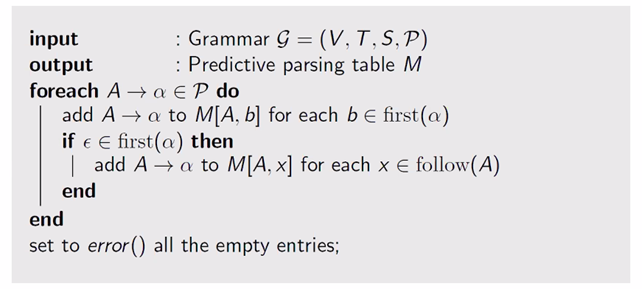
\includegraphics[width=.8\textwidth]{algoritmo_parsing-table.png}
    \caption{Algoritmo di costruzione dei una parsing table}
    \label{algoritmo_parsing-table}
\end{figure}
\subimport{assets/pseudocode/}{parsing-table-comp.tex}
Ricordiamo brevemente che le tabelle di parsing ci servono per verificare se una certa parola può essere derivata tramite derivazione canonica da una data grammatica.

L'algoritmo prevede di scorrere tutte le produzioni \(A \to \alpha\) presenti nella grammatica e, per ognuna di queste:
\begin{enumerate}
    \item aggiungere \(A \to \alpha\) in \(M[A, b]\) per ogni \(b\) in first(\(\alpha\));
    \item se  \(\varepsilon \in\) first(\(\alpha\)), aggiungere \(A \to \alpha\) a \(M[A, x]\) per tutti gli \(x\) in follow(\(A\)). 
\end{enumerate}
Una volta terminato questo ciclo, si va a settare il valore \(error()\) in tutte le entry della tabella ancora vuote.

Osserva che follow(\(A\)) può contenere il simbolo \(\$\), ed è questo il motivo per cui nel punto due usiamo \(x\) invece che \(b\); infatti, mentre \(b\) indica terminali, \(x\) serve proprio a far notare che potrebbe esserci \(\$\), che non è un terminale della grammatica, ma il carattere segnalatore della terminazione di una parola.

Alcune note interessanti:
\begin{itemize}
    \item nel nostro caso le caselle di errore saranno lasciate vuote, mentre nell’applicazione effettiva le caselle vuote puntano tutte a routine di errore;
    \item ripetiamo che è possibile finire con l'avere con due entry in una stessa cella; tuttavia, le grammatiche che compongono tabelle con questa forma non sono deterministiche e non appartengono alla classe LL(1), che è la lasse di cui ci interessiamo noi;
    \item le entry multiple nella tabella di parsing si dicono multiply-defined.
\end{itemize}

\subsection{Applicazioni}
Viene proposta ora come esempio al lettore questa grammatica.
\begin{align}
    \label{non-ll1_grammar}
    \mathcal{G}: E &\to E+T \mid T \\
    T &\to T*F \mid F \nonumber \\ \notag
    F &\to (E) \mid id \nonumber  \notag
\end{align}
Saprebbe dire il lettore se la grammatica qui presentata appartiene alla classe LL(1)?

Mentre il lettore riflette su questo quesito può leggere un'altra importante citazione del nostro punto di riferimento, Paola Quaglia, la quale riflette sul senso di incomunicabilità che attraversa i tempi moderni, quel conflitto generazionale di cui tutti, in certo momento della nostra vita e in un certo schieramento, siamo stati attori.
\begin{displayquote}
    "NWY5YTliMmVjMmRhNiwyOS8xMC8yMDIwIDExOjUxLGthbHQxMA==  kaltura ci parla cosi' :-("
\end{displayquote}

Ebbene, per rispondere alla domanda posta in precedenza la grammatica in \ref{non-ll1_grammar} non appartiene alla classe LL(1) e lo si può dimostrare provando a crearne la parsing table.

Si può notare di fatto come first(\(E\)) = first(\(T\)) = first(\(F\)) \(= \{(, id\}\).
Di conseguenza, se seguiamo i passi dell'algoritmo di creazione della parsing table, otteniamo una situazione in cui la casella \(M[E, id]\) contiene sia \(E \to E+T\) che \(E \to T\). Ma su questa grammatica abbiamo anche altre cose da dire.

\section{Grammatiche con ricorsione sinistra}
La grammatica vista sopra \ref{non-ll1_grammar} presenta anche una proprietà (o difetto) molto interessante, chiamata ricorsione sinistra:
\begin{definition}
    Una grammatica presenta ricorsione sinistra (left recursive grammar) se, per qualche \(A\) e \(\alpha\), \(A \Rightarrow^* A\alpha\)
\end{definition}

Ad esempio, consideriamo la seguente grammatica:
\begin{align*}
    S &\to B \mid a \\
    B &\to Sa \mid b
\end{align*}
Questa grammatica è ricorsiva a sinistra, perché possiamo ottenere una derivazione del tipo: \(S \Rightarrow B \Rightarrow Sa\).

\subsection{Grammatiche con ricorsione sinistra immediata}
Se osserviamo la grammatica \ref{non-ll1_grammar}, ci rendiamo conto immediatamente che presenta ricorsione sinistra, dato che possiamo espandere un numero indefinito di volte la produzione \(E \to E+T\) ed ottenere una sequenza di derivazioni come la seguente:
\begin{equation*}
    E \Rightarrow E+T \Rightarrow E+T+T \Rightarrow E+T+T+T \Rightarrow \dots
\end{equation*}
Ma non finisce qui: infatti, questa grammatica presenta, per la precisione, la caratteristica di ricorsione immediata sinistra (\emph{immediately left recursive grammar}), ovvero presenta una produzione in forma \(A \to A\alpha\).

Presentiamo ora un lemma sulle grammatiche con ricorsione sinistra.
\begin{lemma}\label{ll1-leftrec}
    Se una grammatica \(\mathcal{G}\) presenta ricorsione sinistra, immediata o no che sia, allora la tal grammatica \(\mathcal{G}\) \emph{non} appartiene alla classe LL(1).
\end{lemma}
Una volta venuti a conoscenza di questo lemma, è lecito chiedersi se tali grammatiche proprio non siano riducibili a grammatiche di tipo LL(1) per fare in modo da poterle analizzare in maniera deterministica (e di conseguenza più efficiente).

\subsection{Eliminazione della ricorsione sinistra immediata}
In molti casi è effettivamente possibile eliminare la ricorsione sinistra. 
Proviamo a capire l'intuizione da seguire per ottenere una grammatica LL(1) da una con ricorsione sinistra; per farlo, aiutiamoci tentando di risolvere tale problema per la seguente grammatica d'esempio:
\begin{equation}
    \label{left-recursive_grammar}
    A \to A \alpha \mid \beta \textrm{  con  } \alpha \neq \varepsilon \land \beta \neq A \gamma
\end{equation}
Di fatto, se valesse \(\alpha = \varepsilon\), allora la grammatica sarebbe solo scritta male e non sarebbe quindi left recursive.

\subsubsection{Intuizione}
Per aiutarci a trovare un'idea, possiamo aiutarci andando a tracciare un albero piuttosto grezzo che rappresenti, più o meno, quello che sta succedendo se cerchiamo di derivare lo schema \ref{left-recursive_grammar}:
\begin{figure}[H]
    \centering
    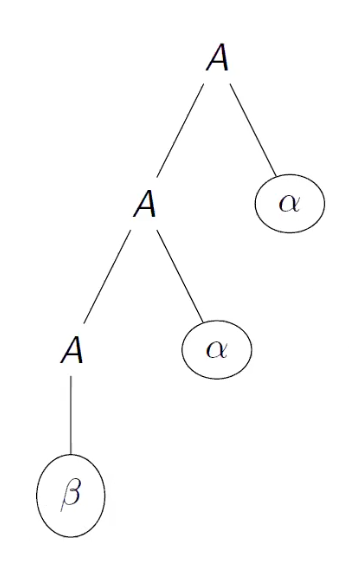
\includegraphics[width=.25\textwidth,keepaspectratio]{lrremove-intuition_1.png}
    \caption{Rappresentazione ad albero del problema}
    \label{lrremove-intuition_1}
\end{figure}
Questa figura non è un vero e proprio albero di derivazione, ma ci permette di capire una cosa: quello che noi vogliamo fare è modificare la struttura dell'albero, quindi le produzioni della grammatica, e al contempo mantenere inalterata la frontiera dell'albero. Potremmo ottenere questo risultato aggiungendo un nuovo non-terminale alla grammatica, in modo da eliminare l'elemento ricorsivo della produzione; idealmente, vorremmo ottenere un risultato di questo tipo:
\begin{figure}[H]
    \centering
    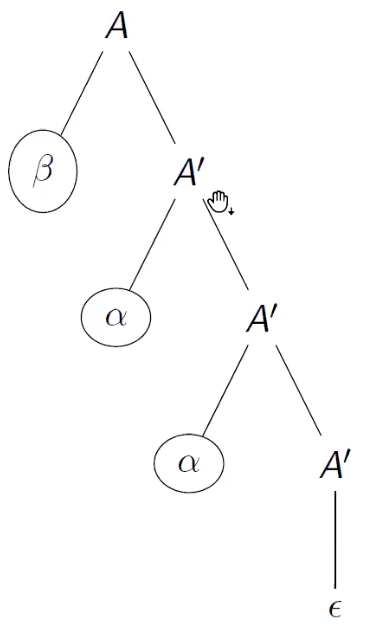
\includegraphics[width=.25\textwidth,keepaspectratio]{lrremove-intuition_2.png}
    \caption{Rappresentazione della nostra intuizione}
    \label{lrremove-intuition_2}
\end{figure}

\subsubsection{Soluzione formale}
A questo punto possiamo scrivere formalmente la nostra strategia per l'eliminazione della ricorsione sinistra immediata: data una produzione del tipo:
\begin{equation*}
    A \to A \alpha \mid \beta
\end{equation*}
dove \(\alpha \ne \varepsilon\) e \(\beta \ne A \gamma\), possiamo riscriverla equivalentemente come segue:
\begin{align*}
    A &\to \beta A' \\
    A' &\to \alpha A' \mid \varepsilon
\end{align*}
dove \(A'\) è un non-terminale \emph{fresh} per la grammatica di riferimento; deve essere fresh, quindi aggiunto alla grammatica, perché altrimenti potrebbe interferire con la derivazione di alcune parole nel linguaggio generato dalla stessa grammatica.

\subsubsection{Formulazione generale}
Riformuliamo la precedente strategia, in modo da astrarla al caso più generale possibile rispetto ai body di una certa produzione.

Per eliminare la ricorsione sinistra immediata di una produzione e mantenerne inalterate le eventuali derivazioni, devo considerare la sua forma:
\begin{equation}
    A \to A \alpha_1 \mid \dots \mid A \alpha_n \mid \beta_1 \mid \dots \mid \beta_k
\end{equation} 
dove \(\alpha \ne \varepsilon \;\; \forall j: 1 \le j \le n\) e anche \(\beta_i \ne A \gamma_i \;\; \forall i: 1 \le i \le k\), con la seguente forma:

\begin{align}
    A &\to \beta_1 A' \mid \dots \mid \beta_k A' \\
    A' &\to \alpha_1 A' \mid \dots \mid \alpha_n A' \mid \varepsilon \notag
\end{align}
Andiamo adesso a vedere come (e se) è possibile elminare la ricorsione sinistra anche quando non è immediata.

\subsection{Eliminazione della ricorsione sinistra}
Qui il problema si fa più spinoso, e purtroppo possiamo già anticipare che non sarà un'operazione possibile in tutte le grammatiche, e c'è addirittura il rischio che eliminare la ricorsione sinistra per un certo non-terminale causi la sua comparsa per un altro non-terminale.

In ogni caso, l'idea è di ridurre gli steps della derivazione \(A \Rightarrow^* A \alpha\), in modo da ottenere una produzione di ricorsione sinistra immediata e applicare la tecnica che già conosciamo.

Consideriamo la seguente grammatica:
\begin{align*}
    A &\to Ba \mid b \\
    B &\to Bc \mid Ad \mid b
\end{align*}
Notiamo subito che abbiamo una ricorsione sinistra immediata su \(B\),  ma abbiamo anche una ricorsione sinistra su \(A\), attraverso \(A \Rightarrow Ba \Rightarrow Ada\).

Ci eravamo detti di tentare di ridurre gli steps di derivazione; per cui, quello che facciamo adesso è sostituire i non-terminali coi body delle loro produzioni, ad esempio:
\begin{equation*}
    B \to Ad \textrm{ diventerà } B \to Bad \mid bd
\end{equation*}
Mantenendo inalterate le altre produzioni, ottengo la seguente grammatica:
\begin{align*}
    A &\to Ba \mid b \\
    B &\to Bc \mid Bad \mid bd \mid b
\end{align*}
A questo punto diventa molto semplice eliminare la ricorsione immediata di \(B\) con lo stesso metodo visto in precedenza:
\begin{align*}
    A &\to Ba \mid b \\
    B &\to bdB' \mid bB' \\
    B' &\to cB' \mid adB' \mid \varepsilon
\end{align*}

\subsection{Eliminazione di ricorsione sinistra: efficacia}
Fermiamoci un attimo e facciamo il punto della situazione. Prima di questa ampia digressione sulle grammatiche con ricorsione sinistra stavamo parlando di top-down parsing, giusto? Bramavamo una tabella di parsing senza entries con definizioni multiple, perché questo avrebbe reso il nostro parsing deterministico. Sapevamo che, fintantoché andavamo a considerare delle grammatiche LL(1), avremmo potuto dormire sogni tranquilli; ma il lemma \ref{ll1-leftrec} ci ha detto che le grammatiche con ricorsioni sinistra (sia immediata, sia non immediata) non sono LL(1), per cui abbiamo iniziato a chiederci se fosse possibile eliminare in qualche modo questa proprietà. Ebbene, dopo tanto tempo speso nell'impresa, ci chiediamo: dopo aver eliminato tutte le ricorsioni, abbiamo certezza che la grammatica ottenuta sia LL(1)?

Consideriamo la grammatica delle espressioni aritmetiche, visto che siamo partiti da quella; proviamo ad applicare le nostre regole di eliminazione e vediamo cosa succede.
\begin{align*}
    \label{non-ll1_grammar}
    \mathcal{G}: E &\to E+T \mid T \\
    T &\to T*F \mid F \nonumber \\
    F &\to (E) \mid id \nonumber 
\end{align*}
% TODO mostrare gli steps
E il risultato finale è proprio lei, la grammatica che abbiamo visto nel calcolo dei first/follow!
\begin{align*}
    \mathcal{G'}: E &\rightarrow TE' \\
    E' &\rightarrow +TE' \mid \varepsilon \\
    T &\rightarrow FT' \\
    T' &\rightarrow *FT' \mid \varepsilon \\
    F &\rightarrow (E) \mid id
\end{align*}
Per di più sappiamo questa grammatica è LL(1), quindi tutto a posto? L'algoritmo di eliminazione della ricorsione sinistra garantisce effettivamente di ottenere grammatiche LL(1)?

Per evitare di cadere in ragionamenti induttivi fallaci del tipo 
\begin{equation*}
    \textrm{uh, in questo caso funziona} \implies \textrm{funzionerà in qualsiasi caso, no?}
\end{equation*}
andiamo a vedere un altro caso, considerando quindi una grammatica che genera comunque il linguaggio delle espressioni aritmetiche ma, a differenza della formulazione precedente, è ambigua:
\begin{equation*}
    \mathcal{G}: E \to E + E \mid E * E \mid (E) \mid id
\end{equation*}
Andiamo quindi a eseguire la nostra procedura e otteniamo la seguente grammatica:
\begin{align*}
    \mathcal{G'}: E &\to (E)E' \mid idE' \\
    E' &\to +EE' \mid \ast EE' \mid \varepsilon
\end{align*}
Questa grammatica è LL(1)? Sfortunatamente, se costruiamo la tabella di parsing per questa grammatica, troviamo che la cella [\(E', +\)] contiene due produzioni:
\begin{itemize}[noitemsep]
    \item \(+EE'\);
    \item \(E' \to \varepsilon\).
\end{itemize}

%TODO tabella di parsing

Ne abbiamo un ulteriore conferma se andiamo a calcolare i first/follow per \(E\) e \(E'\):
\begin{figure}[H]
    \centering
    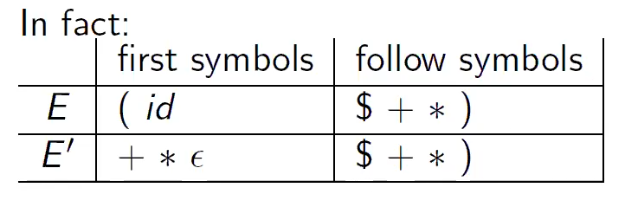
\includegraphics[width=.4\textwidth,keepaspectratio]{fxness-lrremove-fftable.png}
    \caption{Tabella con i first/follow per \(E\) e \(E'\)}
    \label{fxness-lrremove- fftable}
\end{figure}

\paragraph{Conclusione}
Nota bene: non dobbiamo cadere nell'errore di supporre che, magari, la nostra procedura funzioni a meno che non sia lanciata su grammatiche ambigue, perché non ne abbiamo fornito alcuna prova. Da questo  esempio possiamo solamente concludere, a malincuore, che la procedura di eliminazione della ricorsione sinistra \emph{non garantisce} di ottenere delle grammatiche LL(1).

\subsection{Eliminare della ricorsione sinistra elimina l'ambiguità?}
Possiamo però chiederci: la grammatica \(\mathcal{G'}\) che abbiamo ottenuto è ancora ambigua, oppure applicando la nostra procedura ne abbiamo eliminato l'ambiguità? Ricordiamo che l'ambiguità della grammatica di partenza risiedeva nell'impossibilità di esprimere l'associatività degli operatori e la precedenza dell'uno sull'altro\footnote{Si riveda a \ref{sec:ambguity} in caso servisse un ripasso.}. 

Sfortunatamente, riusciamo a trovare senza troppi problemi due derivazioni rightmost che ci portano a ottenere la medesima stringa \(id + id * id\):
\begin{align*}
    E &\Rightarrow idE' \Rightarrow id + EE' \Rightarrow id + E * EE' \Rightarrow id + E * E \\
        &\Rightarrow id + E * idE' \Rightarrow id + E * id \Rightarrow id + idE' * id \\
        &\Rightarrow id + id * id 
    \\ \\
    E &\Rightarrow idE' \Rightarrow id + EE' \Rightarrow id + E \Rightarrow id + idE' \\
        &\Rightarrow id + id * EE' \Rightarrow id + id * E \Rightarrow id + id * idE' \\
        &\Rightarrow id + id * id  
\end{align*}

Possiamo convincerci di questo risultato anche seguendo un altro procedimento, ossia tracciando un albero di derivazione parziale per la nostra grammatica:
\begin{figure}[H]
    \centering
    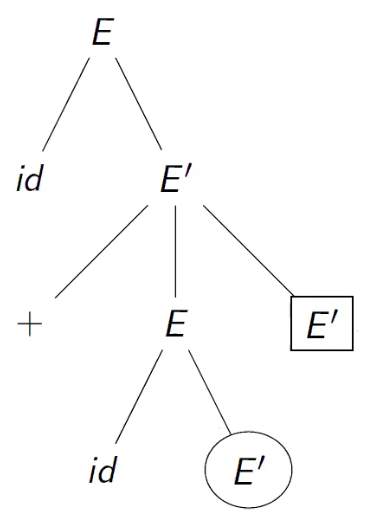
\includegraphics[width=.25\textwidth,keepaspectratio]{fxness-lrremove-ambiguity_1.png}
    \caption{Albero di derivazione parziale per \(\mathcal{G'}\)}
    \label{fxness-lrremove- ambiguity_1}
\end{figure}
A questo punto notiamo subito che, per ottenere la parola \(id + id * id\), possiamo completare questo albero parziale sostituendo i nodi marcati con i seguenti sottoalberi:
\begin{figure}[H]
    \begin{minipage}[b]{0.4\textwidth}
        \centering
        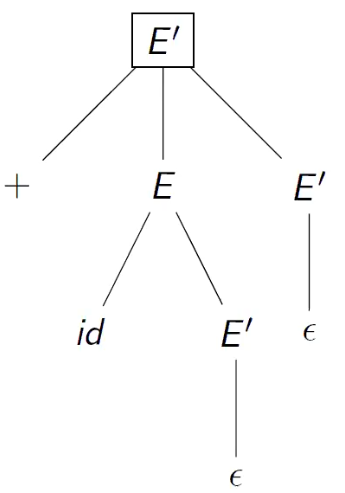
\includegraphics[width=.35\textwidth,keepaspectratio]{fxness-lrremove-ambiguity_2_1.png}
        \subcaption{}
        \label{fxness-lrremove- ambiguity_2_1}
    \end{minipage}
    \hfill
    \begin{minipage}[b]{0.4\textwidth}
        \centering
        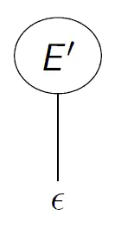
\includegraphics[width=.15\textwidth,keepaspectratio]{fxness-lrremove-ambiguity_2_2.png}
        \subcaption{}
        \label{fxness-lrremove- ambiguity_2_2}
    \end{minipage}
    \caption{Completamento di \ref{fxness-lrremove- ambiguity_1}, versione 1}
    \label{fxness-lrremove- ambiguity_2}
\end{figure}
Ma, allo stesso identico modo, potremmo completare lo stesso albero parzial e ottenere la stessa identica parola sostituendo gli stessi nodi con questi due diversi sottoalberi:
\begin{figure}[H]
    \begin{minipage}[b]{0.4\textwidth}
        \centering
        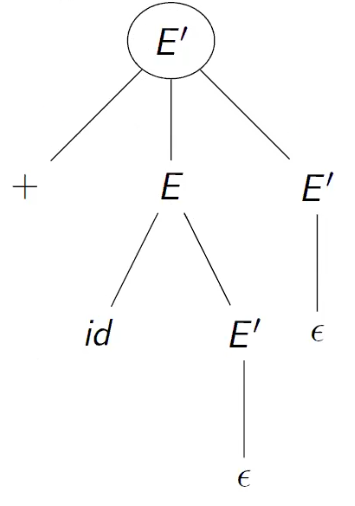
\includegraphics[width=.35\textwidth,keepaspectratio]{fxness-lrremove-ambiguity_3_1.png}
        \subcaption{}
        \label{fxness-lrremove- ambiguity_3_1}
    \end{minipage}
    \hfill
    \begin{minipage}[b]{0.4\textwidth}
        \centering
        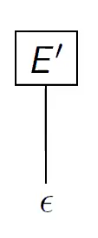
\includegraphics[width=.15\textwidth,keepaspectratio]{fxness-lrremove-ambiguity_3_2.png}
        \subcaption{}
        \label{fxness-lrremove- ambiguity_3_2}
    \end{minipage}
    \caption{Completamento di \ref{fxness-lrremove- ambiguity_1}, versione 2}
    \label{fxness-lrremove- ambiguity_3}
\end{figure}

\paragraph{Conclusione}
Anche qui, non possiamo fare altro che concludere che applicare la procedura di eliminazione della ricorsione sinistra su una grammatica ambigua \emph{non} ne elimina l'ambguità.

\section{Fattorizzabilità Sinistra}
Consideriamo ora la grammatica \(\mathcal{G}: S \rightarrow aSb \mid ab\), che ormai ben conosciamo: questa grammatica ci permette di denotare, ad esempio, un linguaggio composto da parentesi annidate. Quello che non sapevamo è che non è una grammatica LL(1): ce ne possiamo accorgere calcolandone i first(\(S\)), dal momento che l'unico elemento appartenente a questo insieme, nel caso delle due produzioni, risulta infatti essere il non-terminale \(a\); questo vuol dire che, applicando l'algoritmo per la generazione della tabella di parsing predittivo, ci troveremo con due produzioni nella posizione \(M[S, a]\).

Il punto è che \(\mathcal{G}\) può essere \textbf{fattorizzata a sinistra}; in generale, una grammatica è fattorizzabile a sinistra quando:
\begin{itemize}
    \item ci sono almeno due produzioni che hanno lo lo stesso non-terminale come driver;
    \item possiedono un prefisso comune nel body.
\end{itemize}
Nel caso precedente, ad esempio, vi sono due produzioni che hanno \(S\) come driver e \(a\) come prefisso. Rispetto a tutto ciò, analogmente alle grammatiche con ricorsione a sinsitra, abbiamo un lemma.

\begin{lemma}
    Se la grammatica \(\mathcal{G}\) può essere fattorizzata a sinistra, allora sicuramente \(\mathcal{G}\) non è \(LL(1)\).    
\end{lemma}

\subsection{Strategia}
Non possiamo quindi fare a meno di chiederci, di nuovo, sossiamo modificare le produzioni della grammatica in modo da non avere più produzioni per un singolo prefisso, ed evitare quindi di trovarci una tabella di parsing con entries multiple defined.

L'idea che sta alla base della strategia che si utilizza per la fattorizzazione sinistra è quella di rimandare il più possibile la scelta delle produzioni con lo stesso prefisso. Quindi, data una grammatica che ha due produzioni con lo stesso driver e con un prefisso comune, quello che si fa è rimpiazzare la produzione iniziale:
\begin{equation*}
    A \rightarrow \alpha \beta_1 \mid \alpha \beta_2  
\end{equation*}
andando a sostituirla con due produzioni di questo tipo:
\begin{align*}
    A &\rightarrow \alpha A' \\
    A' &\rightarrow \beta_1 \mid \beta_2        
\end{align*}
Dove \(A'\) è un nuovo non-terminale fresh, naturalmente.

Nel caso della prima grammatica non vi può essere determinismo nell'espansione data da \(A\), perché sceglieremo l'espansione indipendentemente dalla lettera successiva a quella considerata correntemente; ad esempio, se potessi sapere che il prossimo simbolo sarà una \(b\), allora non avrei dubbi su cosa scegliere.

\subsection{Algoritmo di fattorizzazione a sinistra}
Il tipo di trasformazione che possiamo fare ad una grammatica generica in modo da rimuovere questi prefissi comuni mantenendo il linguaggio è espresso dal seguente algoritmo: 

\begin{figure}[H]
    \centering
    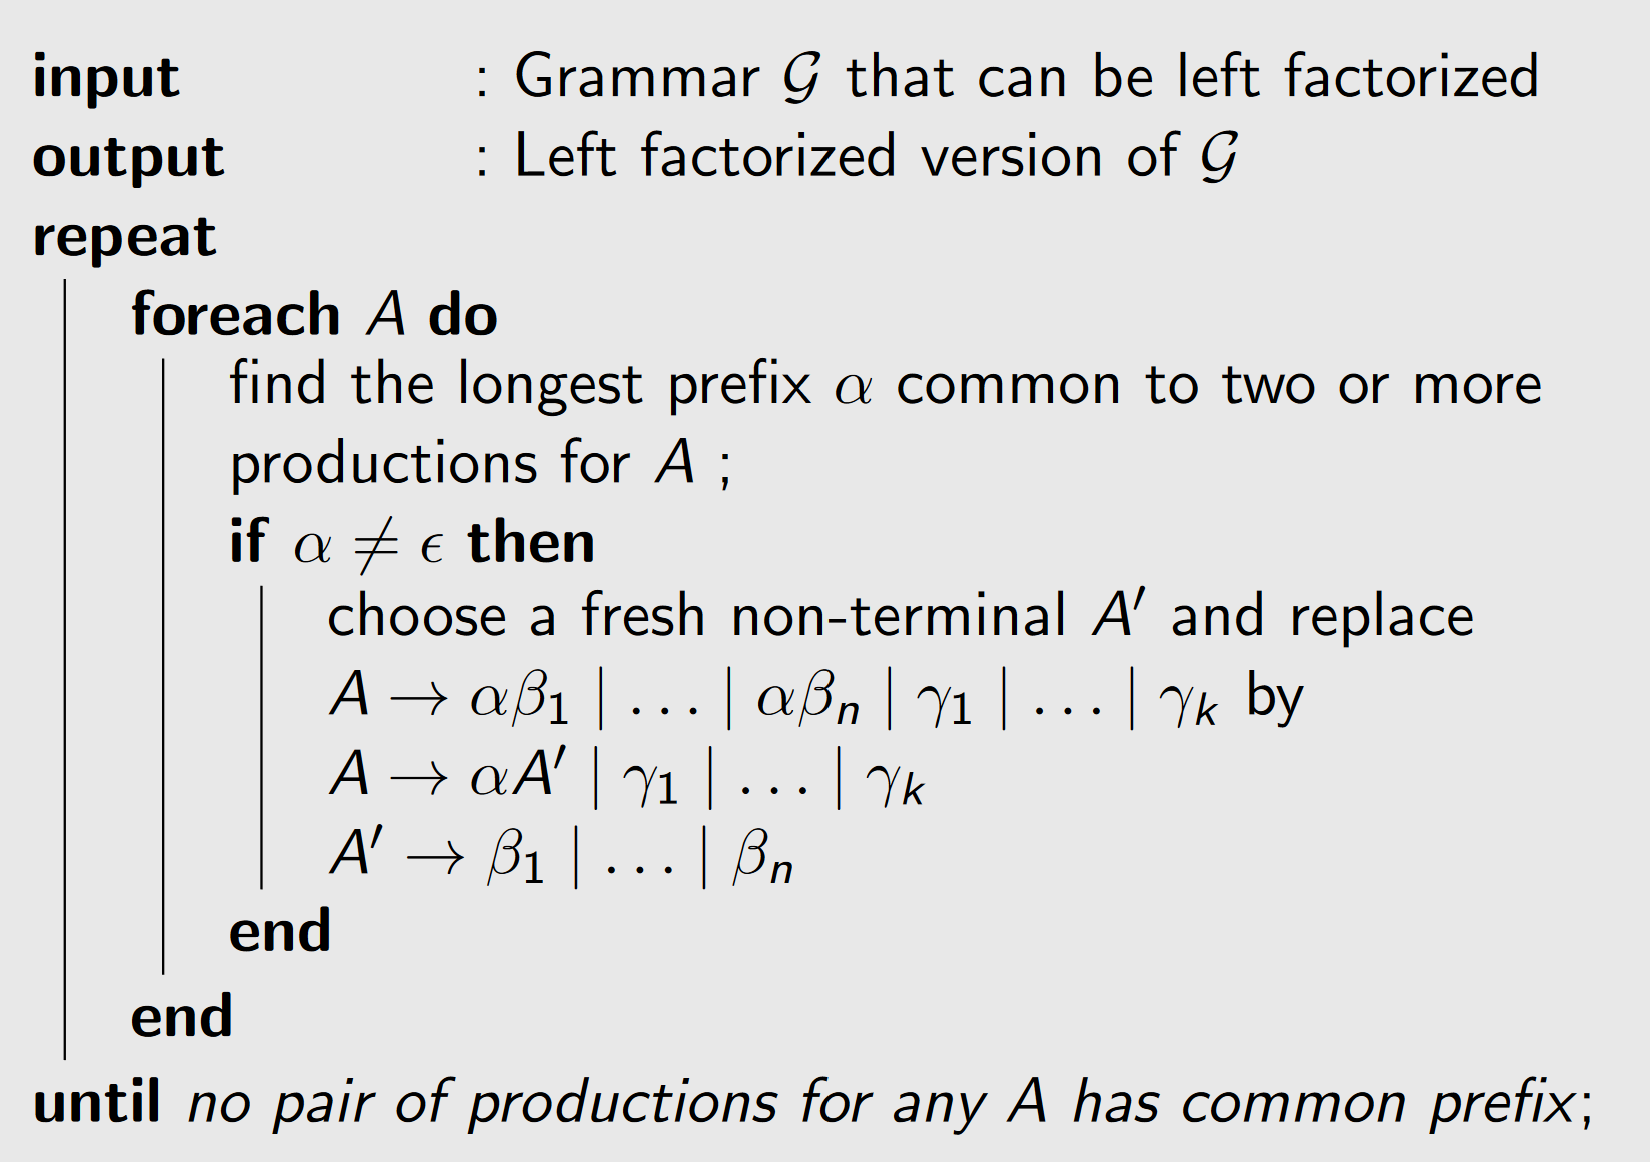
\includegraphics[width=.7\textwidth,keepaspectratio]{leftFactorizationAlgorithm.png}
    \caption{leftFactorizationAlgorithm}
    \label{leftFactorizationAlgorithm}
\end{figure}
\subimport{assets/pseudocode/}{left-fact.tex}

L'idea è che, data in input una grammatica che può essere fattorizzata a sinistra, per ogni non-terminale della grammatica si trova ilpiù lungo prefisso (\(\alpha\)) comune a due o più produzioni aventi lo stesso driver: se un prefisso \(\alpha\) con questa caratteristica esiste, allora viene scelto un nuovo non-terminale e vengono sostituite le produzioni di \(A\) nella forma: 
\begin{equation*}
    A \rightarrow \alpha \beta_1 \mid ... \mid \alpha \beta_n \mid \gamma_1 \mid \gamma_n
\end{equation*}
con le seguenti produzioni: 
\begin{align*}
    A &\rightarrow \alpha A' \mid \gamma_1 \mid \ldots \mid \gamma_n \\
    A' &\rightarrow \beta_1 \mid \ldots \mid \beta_n
\end{align*}
Tale operazione viene ripetuta finché non ci sono più produzioni con un prefisso comune: questo vuol dire che non basta una semplice iterazione di tipo \texttt{foreach} per eliminare i prefissi comuni, ma è necessario esaminare tutte le produzioni, anche dopo che sono stati rimossi dei prefissi; questo perché, naturalmente, è possibile che si generino dei nuovi prefissi a seguito della rimozione dei primi, per cui è opportuno ripetere la procedura finché nessun nuovo prefisso viene trovato.

\paragraph{Considerazioni sull'efficacia}
Vediamo se tale algoritmo risolve il problema che avevamo precedentemente sollevato, ossia se questo impedisca la generazione di entries a definizione multipla nella tabella di parsing. Scopriamolo eseguendo la fattorizzazione sulla nostra fida \(\mathcal{G}: S \to aSb \mid ab\), da cui otteniamo:
\begin{align*}
    \mathcal{G}': S &\rightarrow aS' \\
    S' &\rightarrow Sb \mid b
\end{align*}

Ma quindi, questa \(\mathcal{G}'\) che abbiamo appena ottenuto è una grammatica \(LL(1)\)? Se andiamo a calcolarne i first/follow, troviamo che sono una cosa di questo tipo:
\begin{itemize}
    \item first(\(S\)) = \(\{a\}\) e follow(\(S\)) = \(\{\$, b\}\);
    \item first(\(S'\)) = \(\{a, b\}\) e follow(\(S'\)) = \(\{\$, b\}\).
\end{itemize}
Per cui la tabella di parsing viene costruita come segue:
\begin{table}[h]
    \centering
    \subimport{assets/tables/}{topDownParsingAfterFactorization.tex}
    \caption{Top Down Parsing Table - Dopo fattorizzazione sinistra}
    \label{topDownParsingAfterFactorization}
\end{table}
E quindi tipo è LL(1) sì o no?

\subsubsection{Dangling Else}

Passiamo ora ad esaminare un caso di fattorizzazione sinistra molto famoso nei linguaggi di programmazione e che abbiamo già introdotto, ossia la grammatica ambigua degli \texttt{if} e degli \texttt{else}:
\begin{equation*}
    S \rightarrow \; \textrm{\texttt{if}} \; b \; \textrm{\texttt{then}} \; S \mid \textrm{\texttt{if}} \; b \; \textrm{\texttt{then}} \; S \; \textrm{\texttt{else}} \; S \mid c  
\end{equation*}
Questa grammatica, una volta fatta passare nell'algoritmo di fattorizzazione sinistra,diventa:
\begin{align*}
    S &\rightarrow \textrm{\texttt{if}} \; b \; \textrm{\texttt{then}} \; SS' \mid c \\
    S' &\rightarrow \textrm{\texttt{else}} \; S \mid \varepsilon
\end{align*}
Quindi, la nuova grammatica ottenuta è LL(1)? Calcoliamone i first/follow: 
\begin{itemize}
    \item first(\(S\)) = \(\{\)if \(b\) then, \(c\}\) e follow(\(S\)) = \(\{\$, else\}\)
    \item first(\(S'\)) = \(\{else, \varepsilon\}\) e follow(\(S'\)) = \(\{\$, else\}\)
\end{itemize}  
In questo caso la grammatica risultante non è \(LL(1)\), perché in \(M[S', else]\) ci sono due produzioni: si può infatti osservare che 
\begin{equation*}
    M[S', \textrm{\texttt{else}}] = S' \rightarrow \textrm{\texttt{else}} \; S, \; \textrm{in quanto} \; \textrm{\texttt{else}} \in \textrm{first}(\textrm{\texttt{else}} \; S')
\end{equation*} 
e, allo stesso tempo, abbiamo anche chiederci
\begin{equation*}
    M[S', \textrm{\texttt{else}}] = \varepsilon, \; \textrm{in quanto} \; \textrm{\texttt{else}} \in \textrm{follow}(S')
\end{equation*}
Abbiamo anche un altro modo per constatare che la nostra grammatica rimane ambigua, ossia andando a vedere il seguente albero di derivazione:
\begin{figure}[H]
    \centering
    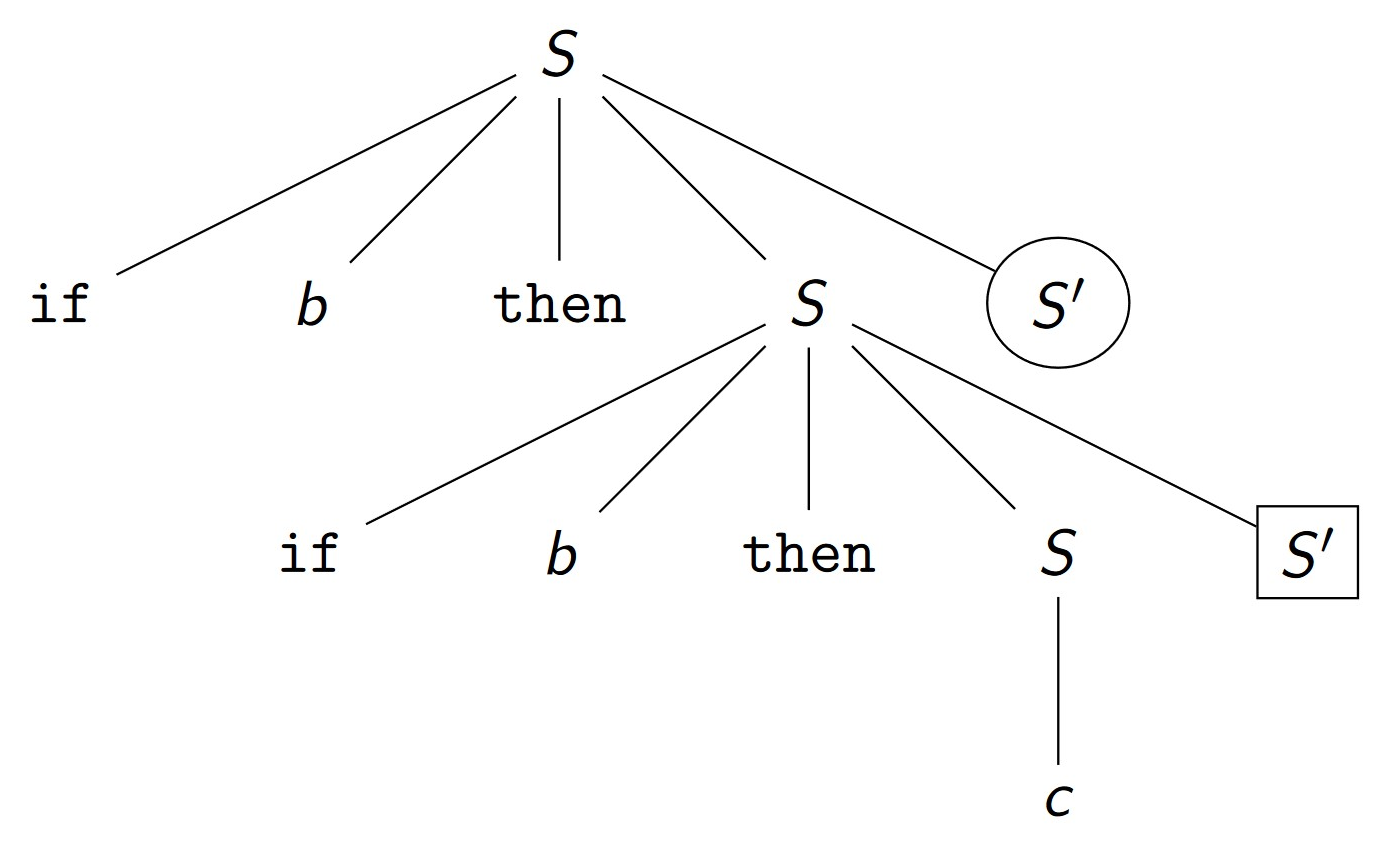
\includegraphics[width=.7\textwidth,keepaspectratio]{leftFactorizationAmbiguity.png}
    \caption{leftFactorizationAmbiguity}
    \label{leftFactorizationAmbiguity}
\end{figure}

Si può infatti notare che in un caso è possibile scegliere di sostituire \({S'}_1\) con \(\varepsilon\) e \({S'}_2\) con \texttt{else} \(c\), mentre nell'altro caso è possibile sostituire \({S'}_1\) con \texttt{else} \(c\) e \({S'}_2\) con \(\varepsilon\), ottenendo di fatto la stessa stringa per due alberi di derivazione differenti utilizzando una derivazione leftmost.

Questo problema viene definito \emph{dangling else} e corrisponde a non sapere identificare in maniera certa di quale \texttt{then} sia figlio un determinato \texttt{else}. per risolvere tale problematica vi sono due differenti soluzioni:
\begin{itemize}
    \item proibire il costrutto \texttt{if-then} e sostituirlo con un \texttt{if-then-else}, tecnica che viene impiegata nel caso dei linguaggi funzionali: l'idea è che bisogna avere un ramo in cui il booleano \(b\) sia valutato a true e un altro nel caso in cui sia valutato a false; nel caso in cui l'\texttt{else} dovesse rivelarsi completamente inutile, allora si crea un ramo fittizio;
    \item imporre l'\textbf{innermost binding}, dove si fa corrispondere l'\texttt{else} al \texttt{then} più vicino e non ancora matchato: ovviamente tale soluzione ha senso solo nel caso in cui non si vogliono utilizzare parentesizzazioni.
\end{itemize}
L'innermost binding può anche essere implementato attraverso la definizioni di policy per definire particolari direttive al parser (approfondiremo il discorso quando parleremo di Byson, niente paura), oppure specializzando la grammatica, permettendo solo a coppie di \texttt{then-else} che matchano tra le occorrenze di \texttt{then} e \texttt{else}, ottenendo dunque la grammatica seguente:
\begin{align*}
    S &\rightarrow M \mid U \\
    M &\rightarrow \texttt{if} \; b \; \texttt{then} \; M \; \texttt{else} \; M \mid c \\
    U &\rightarrow \texttt{if} \; b \; \texttt{then} \; S \mid \texttt{if} \; b \; \texttt{then} \; M \; \texttt{else} \; U
\end{align*}

\section{Riepilogo sulle grammatiche LL(1)}
A questo punto dovrebbe essere chiaro che, se una grammatica è
\begin{itemize}
    \item ricorsiva a sinistra \(\lor\)
    \item fattorizzabile a sinistra \(\lor\)
    \item ambigua,
\end{itemize}
allora non è possibile che sia una grammatica \(LL(1)\). Abbiamo quindi un lemma, che fa più o meno così:
\begin{lemma}
    \(\mathcal{G}\) è una grammatica \(LL(1)\) se e solo se, nel caso in cui \(\mathcal{G}\) avesse delle produzioni del tipo \(A \rightarrow \alpha \mid \beta\), allora:
    \begin{itemize}
        \item first(\(\alpha\)) \(\cap\) first(\(\beta\)) = \(\emptyset\);
        \item se \(\varepsilon \in\) first(\(\alpha\)), allora first(\(\beta\)) \(\cap\) follow(\(A\)) = \(\emptyset\) e, viceversa, se \(\varepsilon \in\) first(\(\beta\)), allora first(\(\alpha\)) \(\cap\) follow(\(A\)) = \(\emptyset\)
    \end{itemize}
\end{lemma}
Questo termina la discussione sulle grammatiche \(LL(1)\). Va però detto che tali proprietà sono estensibili alle grammatiche \(LL(K)\); ricordiamo infatti che l'acronimo \(LL\) si riferisce al fatto che la stringa viene letta da sinistra verso destra e che viene applicata un tipo di derivazione leftmost, mentre il numero 1 messo tra parentesi ci dice che il nostro algoritmo di parsing analizzerà un elemento di input alla volta. L'algoritmo si può dunque estendere se scegliamo di controllare un numero arbitrario \(K\) di elementi alla volta: nel complesso, la strategia è analoga; tuttavia, la tabella di parsing prevedrà delle entries in più. 

Ad esempio, nel caso di una grammatica \(LL(2)\) vanno segnalate sulle colonne coppie di simboli terminali; se prendiamo come riferimento la grammatica \(S \rightarrow aSb \mid ab\), avremo sulle colonne le coppie di terminali \(aa\), \(ab\), \(bb\), \(ba\), \(b\$\), \(a\$\), \(\$\$\). In questo caso, avendo la possibilità di vedere due simboli alla volta riuscirei a fare un parsing predittivo deterministico? Sì, perché so per certo che se leggessi \(ab\) dovrei utilizzare la produzione \(S \rightarrow ab\), mentre in tutti gli altri casi \(S \rightarrow aSb\).

\section{Esercizi riassuntivi sulle grammatiche LL(1)}
\subsection*{Esercizio 1}
Sia data la grammatica \(S \rightarrow aSb \mid \varepsilon\) che denota il linguaggio \(\{a^n b^n \mid n \geq 0\}\); questa grammatica è \(LL(1)\)?

Possiamo facilmente calcolare che first(\(S\)) = \(\{a, \varepsilon\}\), così come follow(\(S\)) = \(\{\$, b\}\). 

Per il lemma precedente visto che first(\(aSb\)) \(\cap\) first(\(\varepsilon\)) = \(\emptyset\) e che, nonostante \(\varepsilon \in\) first(\(\varepsilon\)), abbiamo che first(\(aSb\)) \(\cap\) follow(\(S\)) = \(\emptyset\); ciò può essere osservato anche dalla tabella di parsing predittivo:
\begin{table}[h]
    \centering
    \subimport{assets/tables/}{trainingLL1_1.tex}
    \caption{Es 1 - Training LL(1)}
    \label{trainingLL1_1}
\end{table}
Sorprendentemente dunque la grammatica è LL(1).

\subsection*{Esercizio 2}
Consideriamo adesso la seguente grammatica:
\begin{align*}
    S &\rightarrow AbB \mid B \\
    A &\rightarrow cB \mid a \\
    B &\rightarrow A
\end{align*}
La grammatica sopra citata è \(LL(1)\)? Il sospetto è di no, perché a prima impressione i first(\(A\)) sono uguali ai first(\(B\)) e, essendo che nelle produzioni di \(S\) compaiono in prima posizione entrambi i non-terminali discussi, è possibile che si vadano a collocare nella stessa cella. Procediamo per gradi calcolando i first e, se necessario, i follow:
\begin{table}[h]
    \centering
    \subimport{assets/tables/}{trainingLL1_first_2.tex}
    \caption{Es 2: Calcolo First - Training LL(1)}
    \label{trainingLL1_first_2}
\end{table}
Questa grammatica non è dunque \(LL(1)\), perché nella tabella di parsing avrò le produzioni \(S \rightarrow AbB\) e \(S \rightarrow B\) sia nella cella \(M[S, a]\) che in \(M[S, c]\).
\begin{table}[h]
    \centering
    \subimport{assets/tables/}{trainingLL1_2.tex}
    \caption{Es 2: Training LL(1)}
    \label{trainingLL1_2}
\end{table}

\subsection*{Esercizio 3}
Esaminiamo infine questa grammatica:
\begin{align*}
    S &\rightarrow Aa \\
    A &\rightarrow bB \mid c \\
    B &\rightarrow aA \mid \varepsilon
\end{align*}
\begin{table}[h]
    \centering
    \subimport{assets/tables/}{trainingLL1_first_3.tex}
    \caption{Es 3: Calcolo First \& follow - Training LL(1)}
    \label{trainingLL1_first_3}
\end{table}
Si può notare che mi ritroverò con produzioni in \(M[B, a]\), e ciò è osservabile anche per via del lemma enunciato precedentemente: infatti, si ha che \(\varepsilon \in\) first(\(\alpha\)) e first(\(aA\)) \(\cap\) follow(\(B\)) = \(\{a\} \neq \emptyset\).

la tabella risultante è la seguente, e possiamo dedurne che la grammatica non è \(LL(1)\).
\begin{table}[h]
    \centering
	\subimport{assets/tables/}{trainingLL1_3.tex}
    \caption{Es 3: Training LL(1)}
    \label{trainingLL1_3}
\end{table}

\end{document}